\documentclass[12pt,a4paper]{report}

\usepackage{dolgozat}
\usepackage[]{algorithm2e}
\usepackage[breaklinks]{hyperref}
\usepackage{indentfirst}
\hypersetup{breaklinks=true}

\linespread{1.2}

\begin{document}

\pagestyle{empty} %a címlapon ne legyen semmi=empty, azaz nincs fejléc és lábléc

\begin{flushleft}
\textsc{\bfseries Miskolci Egyetem}\\
Gépészmérnöki és Informatikai Kar\\
Alkalmazott Informatikai Intézeti Tanszék
\end{flushleft}

%A fõiskola logoja
{\large
\begin{center}
\vglue 1truecm
\textbf{\huge\textsc{Szakdolgozat}}\\
\vglue 1truecm

\epsfig{file=cimlap/ME_logo.eps, width=4.8truecm, height=4truecm}\\
\textbf{\textsc{Miskolci Egyetem}}
\end{center}}

\vglue 1.5truecm %függõleges helykihagyás

%A szakdolgozat címe, akár több sorban is
{\LARGE
\begin{center}
\textbf{Számítási modellek bemutatása egy FPS játék készítése kapcsán}
\end{center}}

\vspace*{2.5truecm}
%A hallgató neve, évfolyam, szak(ok), a konzulens(ek) neve
{\large
\begin{center}
\begin{tabular}{c}
\textbf{Készítette:}\\
Árva Zoltán\\
Mérnökinformatikus, BSc
\end{tabular}
\end{center}
\begin{center}
\begin{tabular}{c}
\textbf{Témavezető:}\\
Piller Imre, egyetemi tanársegéd
\end{tabular}
\end{center}}
\vfill
%Keltezés: Hely és év
{\large
\begin{center}
\textbf{\textsc{Miskolc, 2017}}
\end{center}}

\newpage


%Feladatkiiras
\begin{flushleft}
\textsc{\bfseries Miskolci Egyetem}\\
Gépészmérnöki és Informatikai Kar\\
Alkalmazott Matematikai Intézeti Tanszék\hspace*{4cm}\hfil \textbf{Szám:}
\end{flushleft}
\vskip 0.5cm
\begin{center}
\large\textsc{\bfseries Szakdolgozat Feladat}
\end{center}
\vskip 0.5cm
Árva Zoltán (B5X5NT) mérnökinformatikus jelölt részére.\newline

\noindent\textbf{A szakdolgozat tárgyköre:} számítógépi grafika, optimalizálás, C++ programozás\newline

\noindent\textbf{A szakdolgozat címe:} Számítási modellek bemutatása egy FPS játék készítése kapcsán\newline

\noindent\textbf{A feladat részletezése:}

\vfill

\noindent\textbf{Témavezetõ:} Piller Imre (egyetemi tanársegéd) \newline

% \noindent\textbf{Konzulens(ek):} (akkor kötelezõ, ha a témavezetõ nem valamelyik matematikai tanszékrõl való; de persze lehet egyébként is)\newline

\noindent\textbf{A feladat kiadásának ideje:}\newline

%\noindent\textbf{A feladat beadásának határideje:}

\vskip 2cm

\hbox to \hsize{\hfil{\hbox to 6cm {\dotfill}\hbox to 1cm{}}}

\hbox to \hsize{\hfil\hbox to 3cm {szakfelelõs}\hbox to 2cm{}}

\newpage

\vspace*{1cm}  
\begin{center}
\large\textsc{\bfseries Eredetiségi Nyilatkozat}
\end{center}
\vspace*{2cm}  

Alulírott Árva Zoltán; Neptun-kód: B5X5NT, a Miskolci Egyetem Gépészmérnöki és Informatikai Karának végzõs mérnök informatikus szakos hallgatója ezennel büntetõjogi és fegyelmi felelõsségem tudatában nyilatkozom és aláírásommal igazolom, hogy "Számítási modellek bemutatása egy FPS játék készítése kapcsán" címû szakdolgozatom/diplomatervem saját, önálló munkám; az abban hivatkozott szakirodalom
felhasználása a forráskezelés szabályai szerint történt.\\

Tudomásul veszem, hogy szakdolgozat esetén plágiumnak számít:
\begin{itemize}
\item szószerinti idézet közlése idézõjel és hivatkozás megjelölése nélkül;
\item tartalmi idézet hivatkozás megjelölése nélkül;
\item más publikált gondolatainak saját gondolatként való feltüntetése.
\end{itemize}

Alulírott kijelentem, hogy a plágium fogalmát megismertem, és tudomásul veszem, hogy
plágium esetén szakdolgozatom visszautasításra kerül.

\vspace*{3cm}

\noindent Miskolc, 2017. év 11. hó 24. nap

\vspace*{3cm}

\hspace*{8cm}\begin{tabular}{c}
\hbox to 6cm{\dotfill}\\
Hallgató
\end{tabular}



\newpage

\noindent 1.

\begin{tabular}{cl}
&szükséges (módosítás külön lapon) \\
A szakdolgozat feladat módosítása& \\
& nem szükséges\\
&\\
\hbox to 4cm{\dotfill}&\multicolumn{1}{c}{\hbox to 5cm{\dotfill}}\\
dátum& \multicolumn{1}{c}{témavezetõ(k)}
\end{tabular}
\vskip1.5mm

\noindent 2. A feladat kidolgozását ellenõriztem:

\vskip1.5mm

\begin{tabular}{l@{\hspace*{4cm}}l}
témavezetõ (dátum, aláírás):& konzulens (dátum, aláírás):\\
\dotfill&\dotfill\\
\dotfill&\dotfill\\
\dotfill&\dotfill
\end{tabular}

\vskip1.5mm

\noindent 3. A szakdolgozat beadható:

\vskip1.5mm

\begin{tabular}{@{\hspace*{1.3cm}}c@{\hspace*{2.1cm}}c}
\hbox to 4cm{\dotfill}&\multicolumn{1}{c}{\hbox to 5cm{\dotfill}}\\
dátum& \multicolumn{1}{c}{témavezetõ(k)}
\end{tabular}

\vskip1.5mm

\noindent 4.
\begin{tabular}[t]{@{}l@{\hspace*{1mm}}l@{\hspace*{1mm}}l@{}}
A szakdolgozat& \hbox to 3.5cm{\dotfill} &szövegoldalt\\
              & \hbox to 3.5cm{\dotfill} &program protokollt (listát, felhasználói leírást)\\
              &\hbox to 3.5cm{\dotfill}   &elektronikus adathordozót (részletezve)\\
              &\hbox to 3.5cm{\dotfill} & \\
              &\hbox to 3.5cm{\dotfill} &egyéb mellékletet (részletezve)\\
              &\hbox to 3.5cm{\dotfill} &\\
\end{tabular}
\newline tartalmaz.

\vskip1.5mm

\begin{tabular}{@{\hspace*{1.3cm}}c@{\hspace*{2.1cm}}c}
\hbox to 4cm{\dotfill}&\multicolumn{1}{c}{\hbox to 5cm{\dotfill}}\\
dátum& \multicolumn{1}{c}{témavezetõ(k)}
\end{tabular}

\noindent 5.

\begin{tabular}{ll}
&bocsátható\\
A szakdolgozat bírálatra& \\
& nem bocsátható\\
\end{tabular}

\vskip1.5mm

\noindent A bíráló neve: \hbox to 8cm{\dotfill}

\vskip4mm

\begin{tabular}{@{\hspace*{1.3cm}}c@{\hspace*{2.1cm}}c}
\hbox to 4cm{\dotfill}&\multicolumn{1}{c}{\hbox to 5cm{\dotfill}}\\
dátum& \multicolumn{1}{c}{szakfelelõs}
\end{tabular}

\noindent 6.
\begin{tabular}[t]{@{}l@{\hspace*{1mm}}l@{\hspace*{1mm}}l@{}}
A szakdolgozat osztályzata& &\\
&a témavezetõ javaslata:& \hbox to 3cm{\dotfill}\\
&a bíráló javaslata:& \hbox to 3cm{\dotfill}\\
&a szakdolgozat végleges eredménye:& \hbox to 3cm{\dotfill}
\end{tabular}

\vspace*{4mm}

\noindent Miskolc, \hbox to 4.5cm{\dotfill} \hspace*{2.5cm}
\begin{tabular}[t]{cc}
\hbox to 6cm{\dotfill}\\
a Záróvizsga Bizottság Elnöke
\end{tabular}


\cleardoublepage
\pagenumbering{gobble}
\tableofcontents
\cleardoublepage
\pagenumbering{arabic}

\newpage

\pagestyle{myheadings}
\pagestyle{fancy}

\clearpage
\setcounter{page}{1}

\Chapter{Bevezetés}
\label{Chap:bevezetes}

Egy FPS (\textit{First-Person Shooter}) játék elkészítése különféle számítási- és optimalizálási problémákat vet fel. A számítógépes grafika és a játékfejlesztés segítségével lehetőség adódott a termelésinformatikához kapcsolódó optimalizálási problémák bemutatására.

Azon számítógépes játékoknak, amelyek célja a minél valószerűbb megjelenítés, számos olyan eleme van, amely optimalizálás nélkül olyan erőforrásigényes lenne, amely a manapság elérhető csúcskategóriás számítógépeken sem futna megfelelően. Ilyen elem például a karakterek mozgásterének definiálása, a lövés során eltalált objektumok metszéspontjának számítása, az ellenfelek viselkedésének szimulálása.

Megjelenítés szempontjából nagyon fontos, hogy a videokártyának megfelelő formátumban, egyben adjuk át a kirajzolni kívánt elemeket, mert így hatékonyabb lesz a megjelenítés, jobban ki lehet használni a rendelkezésre álló erőforrásokat, illetve a magasabb másodpercenkénti képkockaszámot.

A problémakör egyik fontos eleme az ellenfelek bejárható területének kezelése. Tulajdonképpen ez is egyfajta ütközésvizsgálatot jelent a falakra, objektumokra nézve. A dolgozatban bemutatásra kerülnek azon térpartícionálásos megoldások, amelyekkel a számítások gyorsabban, hatékonyabban elvégezhetők.

Az ütközésvizsgálat egy másik tipikus esete az ilyen jellegű játékokban a lövedékek útjának és metszéspontjainak kiszámítása. Ennél például jelentős optimalizációt érhetünk el, ha csak azon objektumokat vesszük figyelembe, amelyek a lövedék haladási irányába esnek.

Az ellenfelek találatainak regisztrálását az optimális teljesítmény érdekében nem közvetlenül a játékos számára látható, komplex geometriára végezzük el, hanem egy egyszerűbbre. Ezen egyszerűbb geometria részletességének meghatározása nagyon fontos tényező, mert ha túl egyszerű, nem lesz pontos a találatok regisztrálása, ha túl komplex, akkor pedig túl nagy lesz az erőforrásigénye.

Az ilyen jellegű játékoknak egy fontos eleme az ellenfelek viselkedésének modellezése. Minden ellenfélnek van egy aktuális célja, amit a különböző környezeti tényezők befolyásolhatnak. Fontos, hogy a játékos úgy érezze, hogy a mesterséges intelligencia ésszerűen cselekszik, ennek megvalósítását is részletezi a későbbiekben a dolgozat.

\Chapter{Problémakör}
\label{Chap:problemakor}

%- Quake, Unreal, Unity, Cry Engine említés szintjén
%- A játékmotorok fő funkciói
%- Miért volt szükség új játékmotor implementálására?

%Problémafelvetés

%- Leírni, hogy melyek azok a funckiók, amelyekre a játékmotorban szükségesek.

%Milyen konkrét problémát old meg?

%- Felsorol néhány gyakori optimalizálási problémát.

%Miért volt szükség az elkészítésére?

%- Lehetőséget adott az optimalizálási problémák vizsgálatára.
%- Aktívan kutatott terület.
%- Az eredmények szemléletesek.

\section{Játékmotorok}

Új játék fejlesztésénél két fő lehetőség adott, az első, hogy választunk egy előre megírt motort, ami a játék alapját adja, illetve ha egyiket sem tartjuk megfelelőnek, akkor írunk egyet saját magunknak. Meglévő motorok például az Unreal engine, Cryengine, Quake engine (ID Tech). Az Unreal engine első változata 1998-ban jelent meg, az első játék, ami ezt használta az Unreal című játék volt. A motor jelenlegi, legújabb verziója a 4.17-es, nagyon sokat fejlődött az évek során. A Cryengine-t először a Far Cry (\ref{fig:farcry} ábra) nevű játéknál használták 2004-ben, a második, illetve harmadik verziót pedig a Crysis trilógiához. Ezen játékok mindegyike a magas, korát megelőző grafikai megjelenésről lett híres, nagyon szép összképet lehet elérni ezzel a motorral. Az általam írt motorhoz a legközelebb a Quake engine (ID tech) 2 és 3 áll.  Ezen motorok, összességében bármelyik megoldást is választjuk, a játékunk fő komponenseinek a háttérszámításait végzik, pl.: lövés pályájának számítása, gravitáció, ütközésdetektálás, billentyűzet és/vagy egérkezelés, hangok, hálózati kommunikáció, animációk, mesterséges intelligencia. A játékmotor kiválasztása vagy megírása után, a következő lépés a játék felépítésének kialakítása a motor adta lehetőségekkel, eszközökkel. Úgy kell választanunk játékmotort, hogy annak funkcióival megvalósítható legyen a játék.

\begin{figure}[h]
\centering
\includegraphics[scale=0.27]{kepek/farcry.png}
\caption{Pillanatkép a Far Cry című játékból (Crytek)}
\label{fig:farcry}
\end{figure}

\section{Miért volt szükség új játékmotor készítésére?}

A saját játékom tervezésekor, át kellett gondolnom, hogy milyen jellegű programot szeretnék írni, annak milyen funkciói lesznek, hogyan tervezem azt megvalósítani. Mint ahogy korábban írtam, úgy kell megválasztani a motort, hogy azzal megvalósíthatók legyenek az általunk elképzelt funkciók. Ebben az esetben egyrészt azért volt szükség új játékmotorra, mert a tervezés során előjöttek olyan ötletek, játékelemek, amik teljesen egyediek ebben a formában. Ilyen például a csapda, ami egy bizonyos idő után jön elő, ha a játékos nem mozdul meg. Másrészt pedig ez lehetőséget adott az optimalizálási problémák vizsgálatára, programfejlesztési (architekturális), optimalizálási feladatok sorát adta.

\section{Lehetséges optimalizálási problémák}

A játékban megvalósítandó elemek között szerepel a lövés, a mesterséges intelligencia, az ütközésvizsgálat, és mindnek megvannak a maga optimalizálási problémái. Ütközésvizsgálatra szükség van a játékos karakterének az ellenfeleknek és a lövéshez is a találatok regisztrálására, pontos helyének számolására. A játéktér háromszögekből áll. A lövés megvalósításához szükségünk van háromszög, és egyenes metszéspontjának számítására, hogy vizualizálható legyen a lövedék becsapódásának helye a talajon, falakon, illetve egyéb játékbeli elemeken. Ez alapjában véve egy matematikai probléma, amit ki kell számoltatni, le kell programozni. Meg kell határozni azt az egyenest, ami azt mutatja meg, éppen merre nézünk, majd vizsgálni kell, hogy az adott egyenes metszi-e a teret alkotó háromszögek egyikét. De mivel több 100000 háromszög és egyenes metszéspontját kellene alap esetben számítani, így ez több optimalizálási problémát is felvet, amit a későbbiekben részletezek.

\section{Az egyedi motorral megvalósított elemek}
\subsection{Mesterséges intelligencia}

Az MI osztálynak elsősorban az a feladata, hogy az ellenfelek egy meghatározott útvonalon mozogjanak, ne menjenek át falakon, menjenek egymásba. A véletlenszerűen lerakott ellenfelet a legközelebbi definiált waypoint-hoz kell irányítani, definiálni kell a célpontot (ami elsődlegesen a játékos), és ki kell számítani a pontokon keresztül vezető legrövidebb útvonalat.

\subsection{Hangok}

Egy játék alapelemeihez hozzátartoznak a hangeffektek, zenék is, amik élvezetessé teszik azt. Egy jól megválasztott zene például nagyon sokat tud javítani a játékélményen. Ezek megszólalásáért az SDL\_mixer felelős, ami lehetővé teszi azt is, hogy több hang egyidőben, átfedésben megszólaljon, és ne várják meg egymást. Ezt a Sound osztályban valósítottam meg. Lehetőség van hangcsatornákat megadni, folyamatos újrajátszást, illetve a hangok egymáshoz viszonyított hangerejét beállítani.

\subsection{Magasságmező}

A játékteret adó domborzatot, a játék egy fekete-fehér, 384x384 pixeles képből számolja ki. Az adott képen minél magasabb egy pont, annál fehérebb, így a fehér adja a legmagasabb, a fekete szín a legalacsonyabb pontot. Ezekből az adatokból vissza lehet számolni a játékos függőleges pozícióját is, illetve az átmeneteket nézve, meredekségnek megfelelően a visszacsúszást. Mindez tehát megadja a játékteret minden szempontból (vizualitás, játékos mozgástere).

\subsection{Konkrét megjelenítés}

A játéktér adatait tehát képből kinyertük, de ez még nem jelenti azt, hogy látjuk is a monitoron. Ehhez a VBO-s (Vertex Buffer Object) kirajzolási módszert választottam, ami a videókártyának a legoptimálisabb adatstruktúrában adja át azt a lehető leggyorsabb kirajzoláshoz.

\subsection{A csapda mint játékelem}

Mindenképp szerettem volna olyan elemet a játékba, ami megkülönbözteti a többi hasonló, aréna jellegű, túlélős játéktól. Az egyik ilyen elem, hogyha a játékos megáll x ideig (az x majd tesztelés során derül ki mi a legoptimálisabb), akkor megjelenik egy csapda, majd leesik, és meghal. Vannak olyan játékok, ahol szimplán az ellenfelek ösztönzik a játékost a mozgásra, de itt konkrétan ki is van kényszerítve. Jelenlegi beállítás:
Ha megáll a játékos 5mp-ig, akkor megjelenik a csapda modell egy hang kíséretében, illetve onnantól nem lehet már pozíciót változtatni, csak az egérrel körbe nézni. Majd még 2mp leteltével már az egeret sem érzékeli, a föld felé fordul a kamera, majd leesik, ekkor ismét egy hangot lehet hallani, és értesül a játékos arról, hogy miért halt meg.

\subsection{A lövés}

Egy ilyen játékban alapelem az is, hogy tudjunk lőni, mivel ez nélkül az egész értelmét veszti. A textúrázott játéktéren ugyan nem látni, de az egész több százezer háromszögből áll. Adott egy irányvektor, ami azt határozza meg, merre fordul épp a játékos, azaz mire néz. Ennek a vektornak a metszéspontját kell vizsgálni a háromszögekkel, hogy találatot meg tudjuk jeleníteni, ami jelen esetben a falon egy lövésnyom. Szóval ki számolja a program a metszéspont x, y, z koordinátáját, majd odailleszt egy lövésnyom textúrát. Az ellenfeleknél szintén metszéspontot kell számolni, csak ott hengerre. Ki lehetne számolni a modellre is közvetlen, de az nagyon lassú lenne, így egy leegyszerűsített alakzatot választottam. Ez az ellenfél ún. hitboxa.

\section{A végső elképzelés}

Mint ahogy a bevezetésben is írtam, egy FPS (First Person Shooter = belső nézetes lövöldözős játék, az adott személy szemszögéből látjuk az eseményeket) játék elkészítését tűztem ki célul. A konkrét elképzelés az, hogy egy aréna jellegű, túlélő játék készüljön el. Nem terveztem online módot, a játékosnak egy mesterséges intelligenciával kell harcolnia. A játékmenet hullámokra lesz osztva, és ahogy halad előre a játékos, annál nehezebbé válik (több és/vagy erősebb ellenfelekkel). Egy hullám akkor ér véget, ha egy előre megadott számú ellenfelet sikerül megölni. A körök között a játékosnak lehetősége nyílik az életerőt és lőszert feltölteni, fejleszteni a fegyverét a teljesítményének megfelelően. A játékmenet nehezítve lesz azzal (azon felül hogy lőnek rá), hogy ha x másodpercig megáll a játékos, akkor azonnal meghal, így mindig mozgásban kell lenni. Ennek az időtartamnak a pontos meghatározása majd a tesztelés során alakul ki. Lehetőség lesz különböző elemeket (ún. power up-okat) felszedni a körök alatt, ami lehet pozitív vagy negatív hatású is. Például adhat/vehet el életerőt, adhat/vehet el lőszert, adhat/vehet el fegyverfejlesztést.

A fentebb leírtak megvalósítása nagyon sok munka és idő. Meg kell valósítani a modellbetöltést textúrázással, az irányítást, fizikát, ütközéskezelést, hitboxot, mesterséges intelligenciát, fényeket, hangokat, árnyékokat.

\Chapter{Komponensek}
\label{Chap:komponensek}

\section{Felhasznált technológiák (C++, SDL)}

Windows operációs rendszeren az általam legjobban megkedvelt program a Microsoft Visual Studio, aminek a 2015-ös verzióját használom. Az évek során nagyon megszoktam a kezelőfelületét, illetve az azon elhelyezkedő gombok, funkciók elérhetősége ebben a leglogikusabbak számomra. A játék megírásához számomra a C++ programozási nyelv tűnt a legmegfelelőbbnek. A mai játékok jó része is ezzel a nyelvvel íródik, mivel „natív” fut a kód a gépen, sokkal jobb választás mint a C\# vagy a Java. Ezalatt azt értem, hogy például egy Java nyelven megírt program futtatásához szükség van egy virtuális gépre, ami tudja értelmezni a fordító által lefordított, még nem gépi kódot. A virtuális gép felelős azért, hogy az adott hardver gépi kódjára forduljon a program. Vannak olyan alkalmazási területek, ahol az utóbbi kettő a jobb, de egy játék esetében az a lényeg minél gyorsabban fusson egy adott gépen, minél több FPS-t (képkocka/másodperc) produkálva.

A képi világ kirajzolásához, illetve a hangok megszólaltatásához az SDL 2.0-t választottam. Az alábbi linken található bővebb leírás, hogy mit is takar pontosan az SDL:

\begin{verbatim}
https://hu.wikipedia.org/wiki/Simple_DirectMedia_Layer
\end{verbatim}

\section{Az alkalmazás fő részei}

A fő részek, és azok kapcsolatainak szemléltetéséhez egy osztálydiagramot készítettem. Ezen megtekinthető a játék felépítése, melyik osztálynak melyik az őse, illetve mely osztályok vannak kapcsolatban egymással. Továbbá feltüntetésre kerültek a kapcsolatokhoz szükséges adattagok, vagy metódusok is.

Ahogy \aref{fig:uml}-es ábrán is látható, a MainGame a játék fő osztálya, ehhez kapcsolódik minden egyéb komponens, és ez felel az ablak inicializálásáért, felhasználói interakciók lekezeléséért. A játékbeli interakciók kezeléséért az Action osztály felelős, ez kezeli az állapotokat, például hogy éppen előre vagy hátra haladunk, ugrunk, vagy futunk. Ennek megfelelően az Action osztály kimenetei alapján a Player végzi el a játékoshoz kapcsolódó cselekvéseket. A MainGame-hez kapcsolódik még közvetlen a Map, a Sound, a MainMenu osztály. 

A Map a játéktér elemeit, és az azokkal kapcsolatos dolgokat foglalja össze. Ide kapcsolódik a DrawHeightMap, amin keresztül betölti, kirajzolja a játék alapját képző domborzatot, és kiszámolja a karakter ütközésvizsgálatához szükséges gradienst is. A VboDrawer és őse a ModelLoader az egyéb játékbeli objektumok (fák, tárgyak) betöltéséért, kirajzolásáért felelős. A BulletCalcs3D a lövéshez kapcsolódó háttérszámításokat végzi, és az adott háromszöggel kapcsolatos x,y,z metszéspontot adja vissza. A Materials osztály az anyagjellemzők beállításáért felelős.

A játék részeit képezik a játékos informálásáért és segítéséért felelős 2D-s elemek is, amelyekért az IngameElements3D osztály felelős. Ez jeleníti meg a célkeresztet, rajzolja ki az életerő és a lőszer mennyiséget jelző textúrát is, amelyeket viszont a Texture osztály tölt be.

A MainMenu osztályban a főmenühöz kapcsolódó elemek vannak, amelyek a menü háttere, illetve a kijelölések lekezelése vizuálisan. Ezeket az elemeket is a VboDrawer és őse a ModelLoader tölti be, rajzolja ki.

A Sound a hangok megszólalásáért, a megfelelő zenék lejátszásáért felelős, az Utils pedig az egyéb, többi osztályba nem tartozó elemeket tartalmazza.

\begin{figure}[h]
\centering
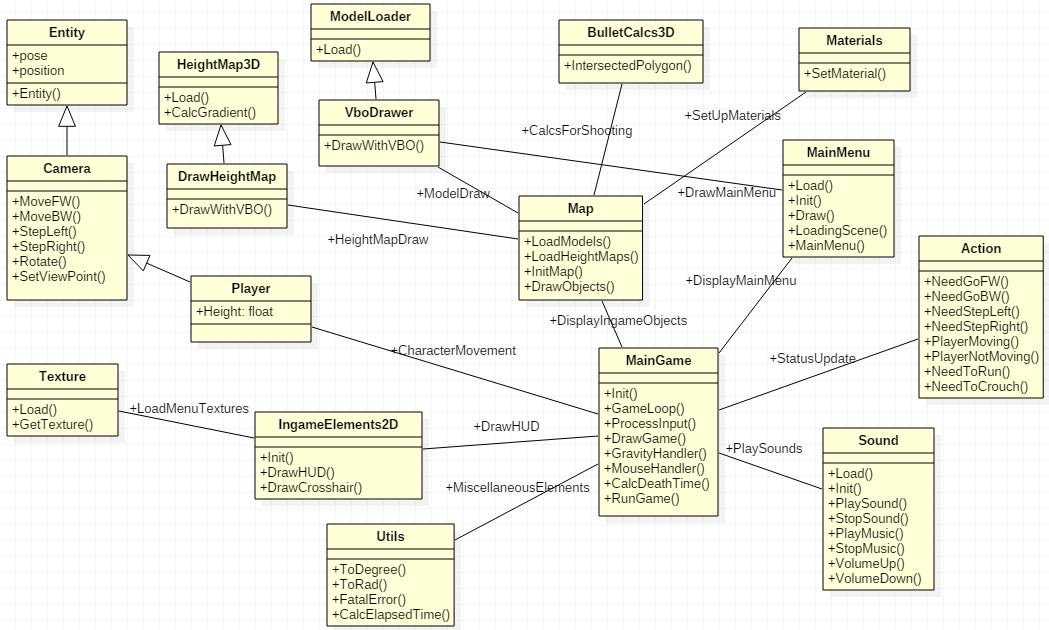
\includegraphics[scale=0.5]{kepek/uml.png}
\caption{A játék felépítése}
\label{fig:uml}
\end{figure}

\subsection{Magasságmező-betöltés, textúrázás}

A játék .obj kiterjesztésű modelleket használ, és ezekre húzza rá a textúrát. A megjelenítéshez VBO-t, azaz Vertex Buffer Object-et használ, ami a modell adatait tárolja, és egyben, a legmegfelelőbb formátumban adja át a videókártyának az optimális sebességért.

Ez egy fekete fehér kép 256 színárnyalatából tud 256 különböző magasságértéket számolni. Mint ahogy korábban is említésre került, a fekete a legalacsonyabb, a fehér a legmagasabb terület, így könnyedén lehet hegyeket illetve völgyeket kialakítani. A játék játszható területének megadásához például \aref{fig:heightmap} ábrán látható képet adhatjuk meg, amiből a magasság értékek számolódnak. A magasságmező textúráját egy külön képfájlból tölthetjük be. Egy ilyen látható \aref{fig:heightmap_texture} ábrán.

\begin{figure}[h]
\centering
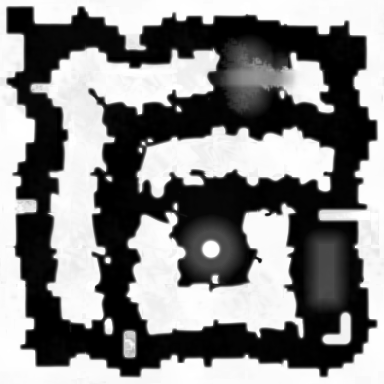
\includegraphics[scale=0.5]{kepek/heightmap.png}
\caption{A magasságmező adatait tartalmazó bitmap}
\label{fig:heightmap}
\end{figure}

\begin{figure}[h]
\centering
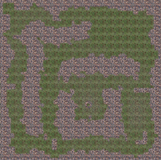
\includegraphics[scale=1.5]{kepek/heightmap_texture.png}
\caption{A magasságmező textúrája}
\label{fig:heightmap_texture}
\end{figure}

\Aref{fig:screenshot} képen pedig a játékban való megjelenés látható. Ez egyben megoldja az ütközéskezelést is, illetve, hogy a túl meredek parton ne lehessen felmenni (lecsúszik róla). A pontokat lineárisan interpolálja, ezzel alkot összefüggő felületet. A textúra ráillesztése is problémás lehet a magasságmezőre, mivel olyan helyeken, ahol túl nagy a gradiens, elnyújtódik. Erre megoldás lehet a multitextúrázás.

\begin{figure}[h]
\centering
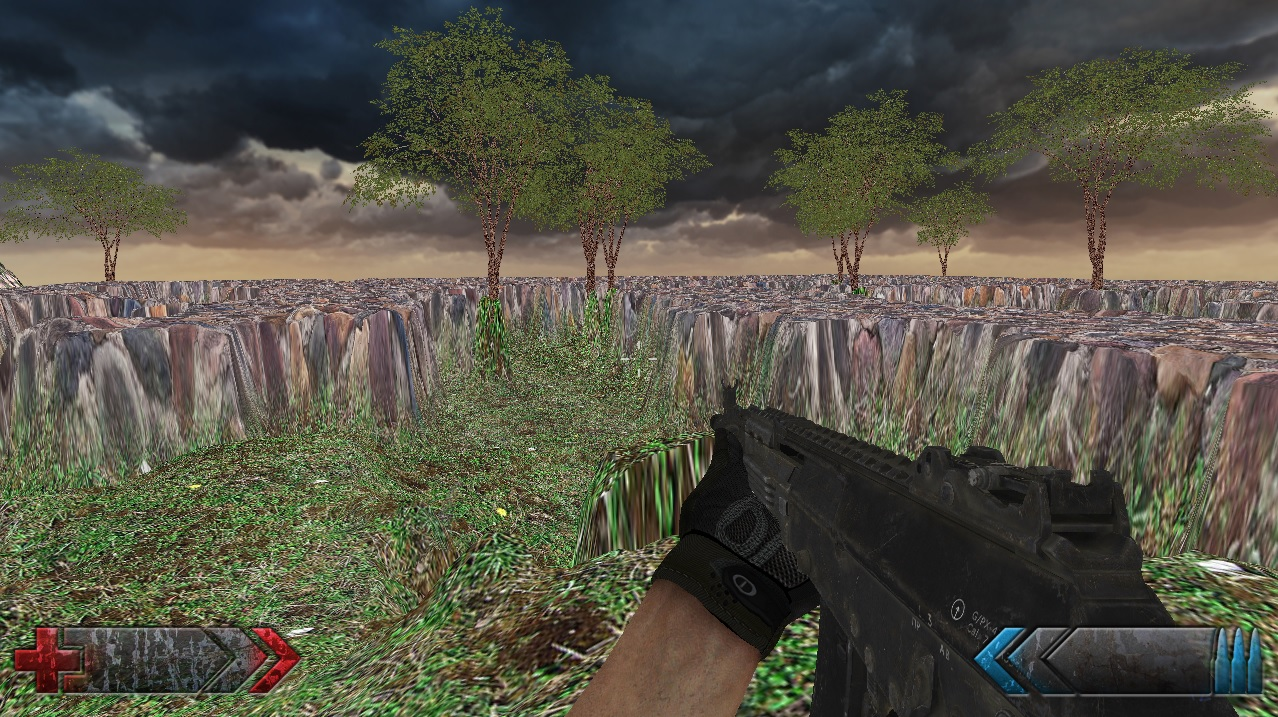
\includegraphics[scale=0.4]{kepek/screenshot.png}
\caption{A megjelenített magasságmező}
\label{fig:screenshot}
\end{figure}

\subsection{A karakter irányítása, fizika}

A játékban egy karaktert irányíthatunk az ő szemszögéből. A karakternek van magassága, x,y,z pozíciója, nézési iránya, amit lát, vagy látunk, a játék szempontjából egy kamera. A kamerához van forgatva a fegyvere, és az ő szemszögéből látható testrészei. Minden cselekedetéhez tartozik egy bool (két állapotú) változó. Például ha tegyük fel előre megyünk, akkor az ehhez tartozó változó „true (igaz)” értéket vesz fel, amihez különböző eseményeket lehet kötni, mint például a kamera előre mozgatását, bizonyos animációk lejátszását. Továbbá a játékosra folyamatosan hat egy gravitációs erő, ami egy float típusú szám. Ezzel lehet elérni azt, hogy ha ugrunk, a játékos visszaessen a talajra.

\subsection{Hangok}

Egyidejűleg több hang lejátszására is szükség lehet, amelyet valamilyen események váltanak ki. A karakter előrehaladása közben egyidejűleg ha lövünk is, már több hangcsatornát igényel, mert így nem várja meg a két hang egymást. Ha csak egy csatorna van, akkor a lépéshangot lejátssza, és csak ez után hallhatjuk a lövést, ami frusztráló, és nem reális. Mivel a játékmenet közben egy hangulatfokozó zene is hallható, ennek lejátszásához, a lépéshanghoz és a lövéshez máris három hangcsatornára van szükség. 

\begin{figure}[h]
\centering
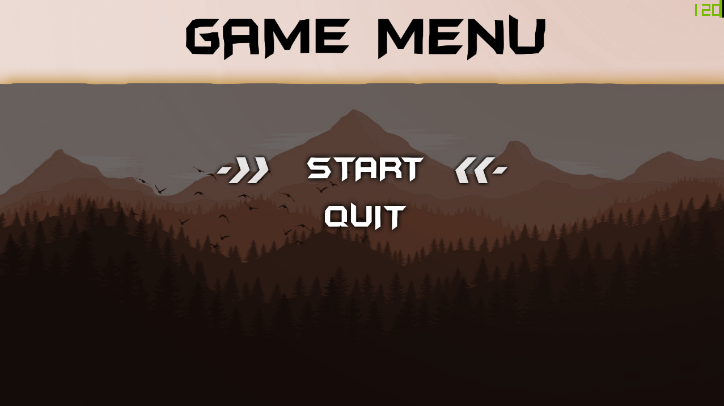
\includegraphics[scale=1.6]{kepek/menu.png}
\caption{A főmenü}
\label{fig:menu}
\end{figure}

\begin{figure}[h]
\centering
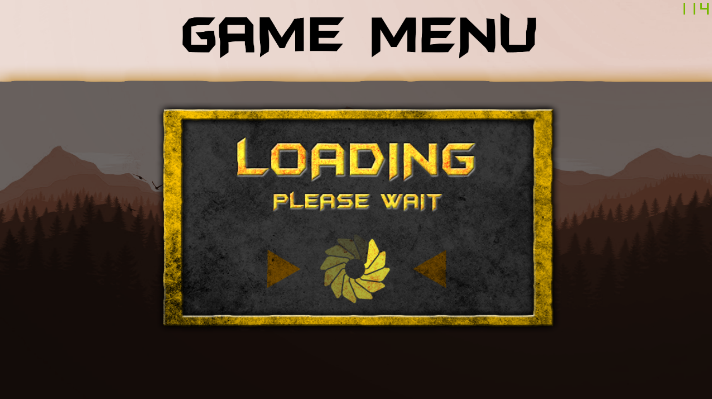
\includegraphics[scale=1.6]{kepek/loading_screen.png}
\caption{Pályabetöltés közben ez látható}
\label{fig:loading}
\end{figure}

\subsection{Lövés}

A lövés háttérszámításai, matematikai kalkulációk is egy külön komponensnek tekinthetők. Első lépés, hogy ki kell számolni a vektort amerre a játékos néz, minden képkockára. Mivel a világ háromszögekből épül fel, ezért ki kell számolni az egyenes háromszöggel való metszéspontját. De mivel több százezer háromszögről beszélünk, ez további optimalizálandó problémákat vet fel, amit a későbbiekben fejtek ki. Bemeneti adatai a játékteret képző háromszögek, illetve a játékos irányvektora, kimeneti adatai pedig a metszéspont x,y,z koordinátája.

\subsection{Mesterséges intelligencia}

Egyjátékos FPS játékról van szó, így mindenféleképp kellett egy, az ellenfelek mozgását irányító mesterséges intelligencia. Ez az egész az A* algoritmusra alapszik. A játék véletlenszerűen, különböző helyekre kirak x mennyiségű ellenfelet, amiknek közeledni kell a játékos felé, különböző kritériumoknak megfelelve. Ezek a kritériumok azért kellenek, mert a pályán vannak játékelemek, amiken nem lehet átmenni, illetve az ellenfelek sem mehetnek egymásba. 

Az alapötlet az, hogy a pályán le lesznek rakva pontok, ún. waypointok, amik csak az ellenfelek számára lesznek láthatók. Ha kikerül egy adott ellenfél a pályára, az első feladata az lesz, hogy megkeresse a hozzá legközelebb eső waypointot. Ezután az A* algoritmus segítségével meghatározza a játékoshoz legközelebb eső waypointhoz vezető legrövidebb utat, végigmegy rajta, majd ha elérte, akkor onnantól a játékos lesz a közvetlen elsődleges célpontja. Mivel a játékos folyamatosan mozog, mindezt másodpercenként legalább 15-30x kell kiszámolni.

Bemeneti adatai a waypointok azok típusaival együtt, kimeneti adata pedig az adott útvonal, hogy az ellenfélnek merre is kell mozognia. Az ellenfél elsődleges célpontja a játékos, de adódhatnak olyan helyzetek amikor előtte egyéb dolgokat helyez előtérbe, mint például az életerő töltés, vagy lőszer felvétel. Itt fontos szerepet kap az ellenfél karakterisztikája, ami szintén bemeneti paraméter.


\section{A játékindítás folyamata}

Első lépésben a játék létrehozza az SDL ablakot, és konkrétan beállítja annak pozícióját, függőleges és vízszintes felbontását, illetve a flageket, pl. a kurzort, teljes képernyő legyen vagy nem.

A második lépés hogy az előtte létrehozott ablakot beállítja aktívra, és OpenGL megjelenítésre. Létre kell hozni egy érvényes OpenGL  kirajzolás kontextust, hogy inicializáljuk a belépési pontokat. Ez használhatóvá teszi az összes elérhető funkciót, amit az OpenGL magban definiáltak. Ezután betölti a főmenü megjelenítéséhez szükséges modelleket, textúrákat.

Harmadik lépésben aktiválja a hangok megszólaltatásáért felelős komponenst, és betölti az összes hangot, zenét.

A negyedik lépésben pedig aktiválja az eseménykezelő komponenst, ami a felhasználótól érkező interakciókat kezeli, majd meghívja a betöltött modelleket kirajzolásra.

A menübe érkezés után a felhasználónak lehetősége nyílik a játékteret betölteni, vagy kilépni. 

A „Start” gombra kattintás után, betöltődik a magasságmező kezelő komponens, a kamera a kezdőpontra pozícionálódik, elkezdődnek a játékmenethez elengedhetetlen háttérszámítások, és egy új zene lejátszása, betöltődnek a játéktér modelljei, elemei, illetve átvált azok kirajzolására. Hogy a játékos informálva legyen, ez idő alatt megjelenik a betöltőképernyő.

\begin{figure}[h]
\centering
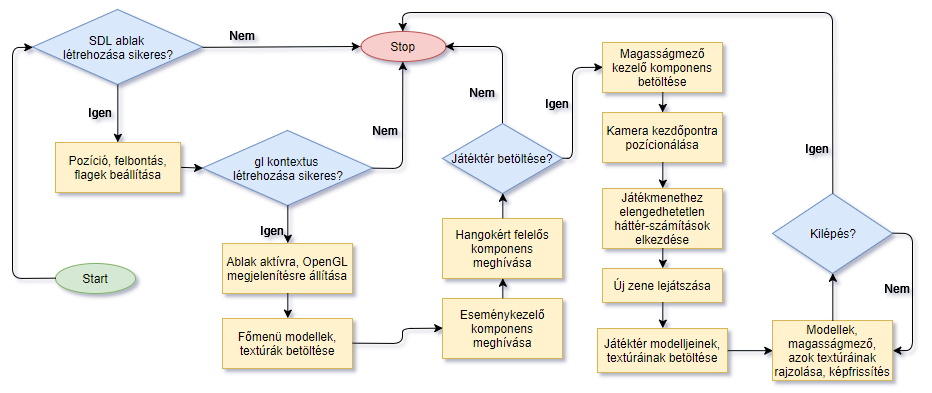
\includegraphics[scale=0.46]{kepek/starting_diagram.png}
\caption{A játék indításának folyamatábrája}
\label{fig:starting}
\end{figure}
\Chapter{Ütközésvizsgálat}
\label{Chap:utkozesvizsgalat}

Ebben a fejezetben az ütközésvizsgálattal kapcsolatos számításokról, optimalizációkról lesz szó. Ütközésvizsgálatra több szempontból is szükség van. Egyrészt, vizsgálni kell, hogy a játékos a játszható területen belül van-e, azaz nem mehet át falakon, tereptárgyakon, nem mehet fel túl meredek emelkedőn. Másrészt, vizsgálni kell, hogy a játékos által leadott lövedék eltalálja-e a domborzatot, tereptárgyakat, jelezni kell a lövedék becsapódását. Harmadrészt regisztrálni kell az ellenfeleket eltaláló leadott lövéseket. A második és harmadik pont nagyon hasonló, de mégis célszerűnek tünt külön kezelni. A magasságmező és az egyéb modellek ütközésvizsgálatának módját azért érdemes külön kezelni, mert a statikus magasságmező esetében másfajta optimalizálási módok állna rendelkezésre, mint az egyéb tereptárgyak, és animált karakterek esetében.

\section{A karakterek ütközésvizsgálata mozgás szempontjából}

Ez a játék szempontjából az egyik legfontosabb elem, mivel ez adja a virtuális világ egyfajta realitását. Az, hogy kirajzoltatunk valamit a képernyőre, még nem jelenti azt, hogy azon nem lehet áthaladni. Konkrétan a Z-buffer felelős azért, hogy a takarási feladatot megoldja, viszont azt úgy képes végrehajtani, hogy közben a kirajzolt objektumok ütközését a lehető legegyszerűbb módon kezeli csak.

A kirajzolás csak a vizualitást adja, a domborzat, a tereptárgyak, a karakterek kinézetét. A játékfejlesztő feladata az, hogy megírja külön az ezekhez szükséges ütközésvizsgálatot. Mivel ez két különálló dolog, egyes helyzetekben adódhatnak olyan problémák, hogy ezek nincsenek szinkronban, tehát látunk valamit amin át lehet menni, vagy nem látunk valamit és mégis megakadunk benne.

A szakdolgozat készítése közben fejlesztett játékmotorban a karakterek és a magasságmező ütközését magasságpontok és az ezek különbségeiből kapott gradiensek számításával oldottam meg. Ez azt jelenti, hogy ha két, egymás mellett lévő pont magasságértéke között túl nagy a különbség pozitív irányba, az falat, vagy túl meredek emelkedőt jelent. Ez a különbség tehát az eredeti felület pontbeli gradiensének numerikus közelítését adja. Ha mérsékelt, vagy nagyon minimális a különbség, akkor arról vagy lecsúszik, vagy csak egyszerűen át lehet ott haladni. Mindezt a beolvasott magasságmezőből számolja, így az ütközésvizsgálat minden új magasságmező esetében automatikusan elérhető.

Jelölje $H$ azt a két változós valós függvényt, amelyet a magasságmezővel közelítünk. Legyen a $\widetilde{H}$ az az interpolációs függvény, amelyeket az interpoláció alappontjaiban felveszik a $H$ értékét. Egy $p \in \mathbb{R}^2$ pozíció esetén a pontbeli gradienst a következő módon közelíthetjük:
$$
\nabla H(p) =
\left( \dfrac{\partial H(p)}{\partial x}, \dfrac{\partial H(p)}{\partial y} \right)
\approx
\left(
\dfrac{\widetilde{H}(p + \delta_x) - \widetilde{H}(p)}{\delta_x},
\dfrac{\widetilde{H}(p + \delta_y) - \widetilde{H}(p)}{\delta_y}
\right),
$$
ahol $\delta_x$ és $\delta_y$ az $x$ és $y$ tengely szerinti tetszőlegesen kis eltolást jelöli.

A gradiens közelítésének ez az egyik legegyszerűbb módja. Előnyös, mivel az interpolt felület pontbeli értékeit egyébként ki kell számítani, illetve a számítási pontosság megfelelő a játékmotor működéséhez.

Ezen felül a gravitáció ami nagyon lényeges, mert a pályának vannak olyan magaslati pontjai, amelyekre fel lehet jutni. Ha egy ilyenre felmegyünk, és nincs semmilyen erő, ami a karaktert a föld felé húzná, akkor felfelé ugyan lekövetné a talajmagasságot, de le már nem tudna esni.

A játékmotor fizikájában egy lefelé ható erő folyamatosan hat a játékosra és ellenfelekre, aminek a küszöbértéke mindig az aktuális talajmagasság. Ugrás esetén a gravitációnál nagyobb, ellenirányú erőt fejt ki a karakter, amely folyamatosan csökken. Ez eredményezi azt, hogy elemelkedik a földtől, egy ponton megáll, majd vissza is esik a talajra. Ez látható \aref{fig:gravity}-es ábrán. A gravitációs erőt az $F_g$ jelöli, a kifejtett erőt pedig az $F_k$.

\begin{figure}[h]
\centering
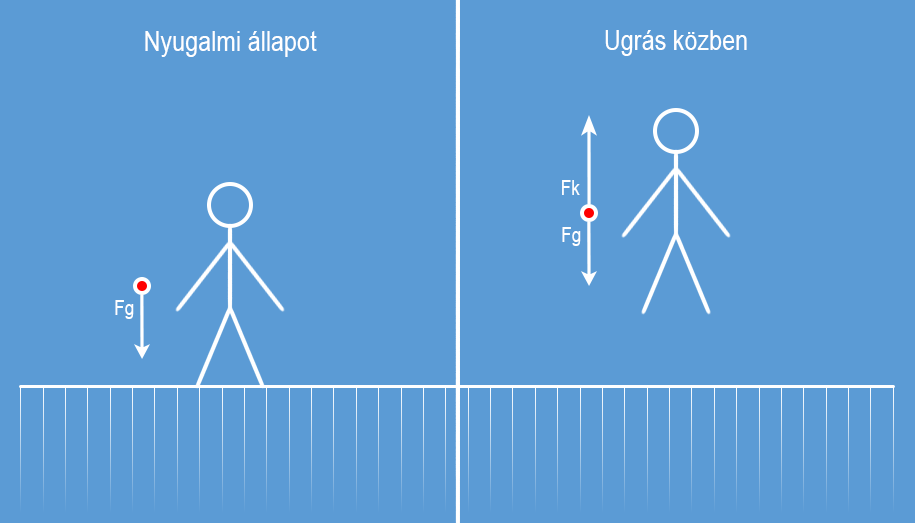
\includegraphics[scale=0.6]{kepek/gravity.png}
\caption{A karakterre ható erők}
\label{fig:gravity}
\end{figure}

A karakter függőleges pozícióját jelöljük $z$-vel. Amennyiben a játékos a magasságmezőn áll, akkor teljesül, hogy $\widetilde{H}(p) = z$. Az $F_g$ gravitációs erőt konstansnak tekintjük. Ennek tipikusan csak $z$ tengely irányú, $0$-tól különböző komponense van. Amennyiben a karakter a magasságmező felett van, úgy a $z$ és az $F_k$ is felírható az idő függvényében $t$ szerint. Egy $\Delta t$ mintavételezési időt feltételezve (ami tipikusan a képkockák kirajzolásai között eltelt idő) a következő összefüggéseket írhatjuk fel:
\begin{align*}
F_k(t + \Delta t) &= F_k(t) + F_g \cdot \Delta t, \\
z(t + \Delta t) &= z(t) + F_k(t) \cdot \Delta t. \\
\end{align*}
Amikor tehát a karakter a magasságmezőre érkezik, akkor az $F_k$ értékét $0$-nak tekinthetjük, a $z$-t pedig a magasságmező adott pontjának értékére állíthatjuk.

A koordinátarendszer és az erők mértékegységének megfelelően szükségünk lehet korrekciós szorzókra, például ha méterben és másodpercben szeretnénk számolni.
 
\section{A domborzat és tereptárgyak üközésvizsgálata a lövés szempontjából}

A domborzattal való ütközésvizsgálat azért fontos, hogy azon keresztül ne lehessen eltalálni az ellenfeleket, illetve ezzel is realisztikussabbá tehetjük a játékot. A nagy poligonszám miatt ez is optimalizációt igényel.

A problémát az egyenes és a háromszög metszéspontjának számítására vezethetjük vissza. A domborzat háromszögeit fekete szegélyekkel láthatjuk \aref{fig:wireframe} ábrán.

\begin{figure}[h]
\centering
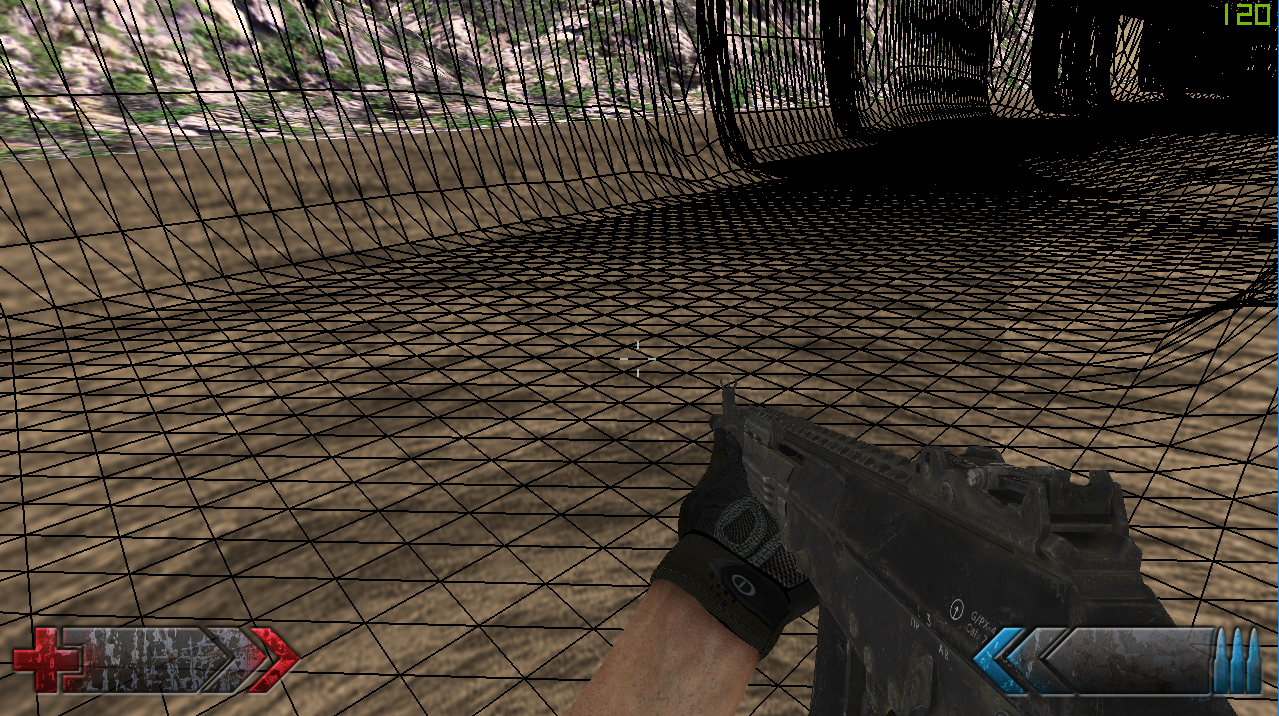
\includegraphics[scale=0.4]{kepek/map_wireframe.png}
\caption{A térkép geometriájának határvonalai}
\label{fig:wireframe}
\end{figure}

\subsection{Program: Ütközésvizsgálat}

Első lépésként, meg kell határozni azt az egyenest, amely azt írja le, amerre néz az adott karakter. Az egyenes megadható két pontjával. Az egyik az adott karakter pozíciójával egyezik meg. A másik, távoli pontot jelen esetben egy, az OpenGL-ben definiált függvényből, a \texttt{GluLookAt} függvényből határozzuk meg, aminek 9 paramétere van. Az első három a karakter jelenlegi pozíciója, a második három azt a pontot írja le merre nézünk (referencia pont), az utolsó három pedig azt határozza meg, hogy melyik tengelyen, és merre néz a felfelé vektor. A 9 paraméter közül a középső háromból lehet a második pontot  meghatározni.

Második lépésként ki kell számolni ennek az egyenesnek a háromszögekkel vett metszéspontját. A háromszögeket a három csúcspontjukkal írjuk le. Kell lennie egy függvénynek, amelynek a háromszög három csúcspontját, és az egyenes két végpontját átadva, visszakapjuk a metszéspont $(x, y, z)$ koordinátáját. A számítás eredményének egy szemléltetését \aref{fig:triangle} ábrán láthatjuk.

\begin{figure}[h]
\centering
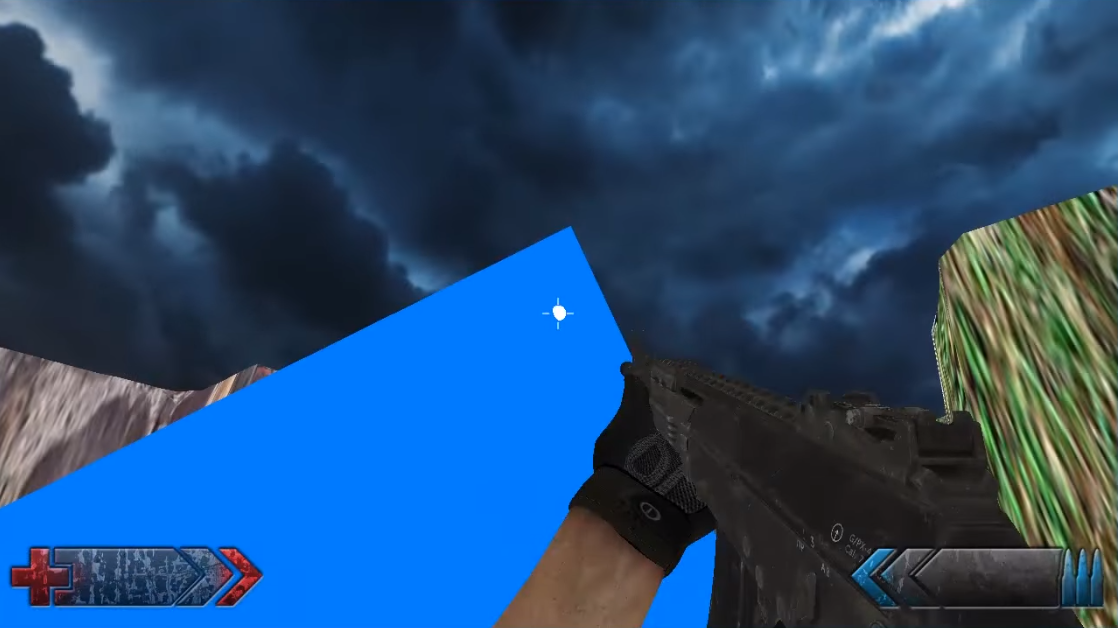
\includegraphics[scale=0.46]{kepek/one_triangle.png}
\caption{Egyenes és háromszög metszéspontja vizualizációval}
\label{fig:triangle}
\end{figure}

A számításhoz a függvény először megvizsgálja, hogy azt a síkot, amelyen a háromszög van, metszi-e az egyenes, ha nem, nem is számol tovább. Ha metszi a síkot, akkor megnézi, pontosan hol metszi azt, melyek a metszéspont $(x, y, z)$ koordinátái. Ez után már csak azt kell vizsgálni, hogy a metszéspont benne van-e a három csúcspontjával leírt háromszögben. Ha igen, akkor visszaadja a metszéspontot.

\section{A játékos, és az ellenfelek ütközésének vizsgálata}

Ennek a működése hasonló, mint a domborzat és tereptárgyak üközésvizsgálatánál, azzal a különbséggel, hogy itt azt kell vizsgálni, hogy az ellenfelek körül lévő, a játékosok számára láthatatlan hengerrel van-e metszéspontja az adott egyenesnek. Ezt a hengert nevezzük jelen esetben \textit{hitbox}-nak. Ennek a megválasztása hatással van egyrészt az ütközésvizsgálat pontosságára, másrészt pedig a számítási időre.

\begin{figure}[h]
\centering
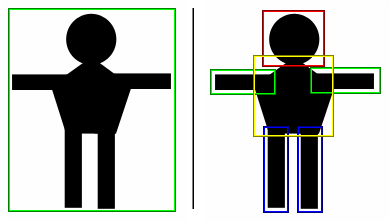
\includegraphics[scale=0.38]{kepek/hitbox.png}
\caption{Különböző részletességű hitbox-ok}
\label{fig:hitbox}
\end{figure}

A hitbox arra szolgál, hogy egy közelítő becslésünk legyen az ütközésvizsgálathoz. Amennyiben eltaláltuk egy objektum \textit{hitbox}-át, úgy meg kell vizsgálni, hogy a benne lévő modellel van-e ütközés. Amennyiben nincs, ugyanazt kell tennünk, mint ha a közelítő alakzattal sem lett volna ütközés.

% Ebben az esetben azért nem a pontos, látható geometriára számoljuk a találatokat, mert annak nagyon nagy erőforrásigénye lenne, ellenben az lenne a legpontosabb, tehát amit látunk, az jelenti a találatot. A találatszámításra használt leegyszerűsített geometria előnye, hogy sokkal kevesebb hátérszámításra van szükség. Viszont mivel nem azt találjuk el, amit látunk, előfordulhatnak kellemetlen, vagy érdekes szituációk. Előfordulhat, hogy úgy találjuk el az ellenfelet, hogy ott valójában nem látunk semmit, vagy ennek ellenkezője, hogy elvileg eltaláljuk, de az a rész nem tartozik a hitbox-hoz.

Online lövöldözős játékoknál további problémát jelenthet a hálózati kommunikációból eredő hosszú válaszidő. Ebben az esetben az ellefél játékosok nem minden esetben azon a pozíción vannak, mint ahol látjuk őket, mivel a számunkra megjelenített helyüket a játékmotor lokálisan becsli. Amennyiben a becslés rossz volt (az ellenfél játékos más irányba mozdult el, mint ahová a kliensünk azt várta volna), az általunk leadott pontos lövést érvénytelennek kell tekinteni.

\section{Optimalizálási módszerek}

Az ütközésvizsgálatra minden képkocka kiszámítása előtt szükség van. Maga a számítás eredeti felírásában nagyon számításigényes, ezért mindenképpen szükséges, hogy ezt valahogyan optimalizáljuk. A következőkben néhány lehetséges optimalizálási módszer kerül bemutatásra.

\subsection{A játéktér szabályos felosztása}

Ez egy olyan módszer, amivel minden egyéb tényezőt figyelmen kívül hagyva felosztjuk a teret egy felosztási részletességet megadva. Meg kell adnunk, hogy melyik objektum, vagy a pályának melyik része melyik térrészben található, ez látható \aref{fig:grid} ábrán. A karakterek ütközésvizsgálatánál elég, ha mindig csak arra a térrészre vesszük figyelembe az ütközést amelyiken épp tartózkodik, de ajánlott a körülötte levő 8 részre is. Lövedék becsapódásának $(x, y, z)$ koordinátáját is kevesebb számítással kaphatjuk meg így, mert csak azokat a térrészeket kell figyelembe venni, amelyek a játékos karakterének irányvektorával metszésben vannak. Előnye, hogy ezt a legegyszerűbb megadni, és ehhez képest elég nagy gyorsulást tapasztalhatunk. Hátránya viszont, hogy mindenhol egyformán osztjuk fel a teret, és lehetnek olyan részek, ahol indokolatlanul sűrű a felosztás. Ilyen például egy nagy mező, minden tárgy nélkül. Azért, hogy a felosztott térrészekben való keresés hatékonyabb legyen, a felosztást egy fa struktúra szerint tesszük meg. A felosztásban szereplő régiók számának logaritmusával lesz majd arányos a keresés lépéseinek a száma.

\begin{figure}[h]
\centering
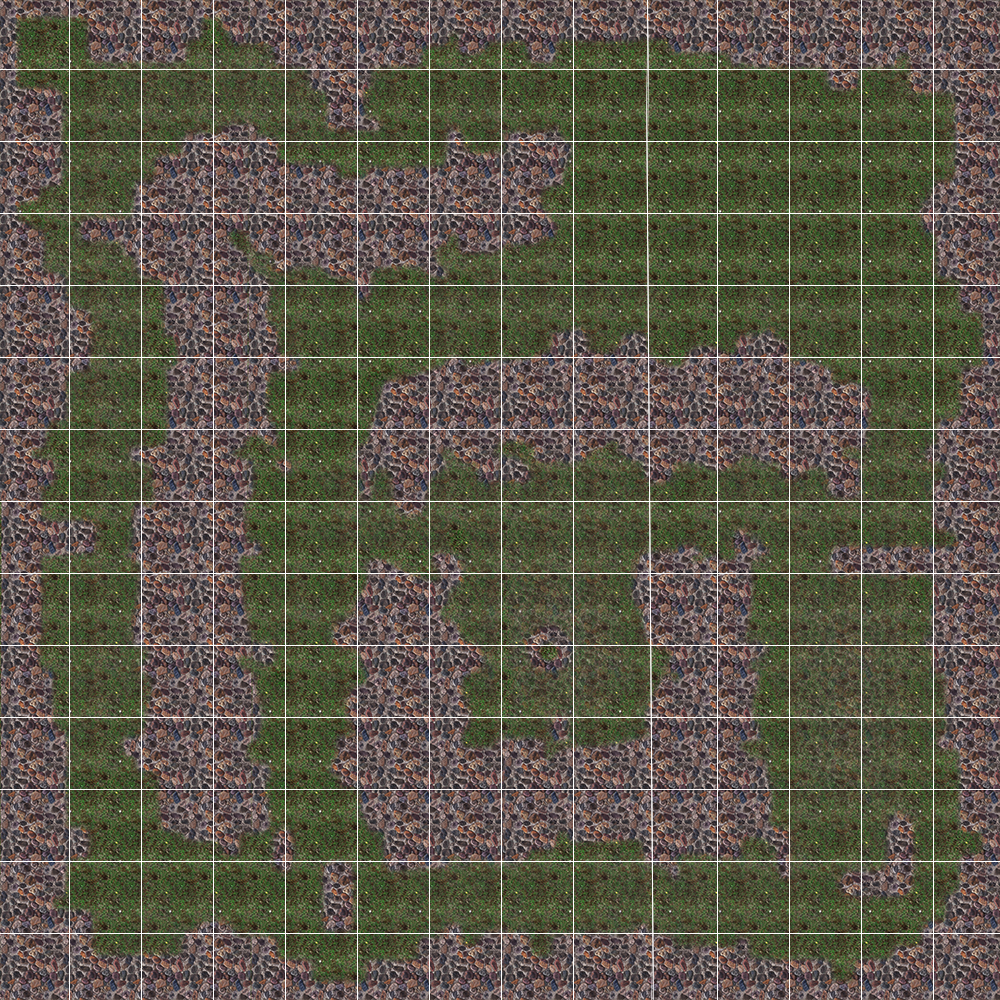
\includegraphics[scale=0.22]{kepek/grid.png}
\caption{A pálya felosztása egyenlő részekre}
\label{fig:grid}
\end{figure}

\subsection{Négyes fa és az oktális fa}

A négyes és az oktális fa ugyanolyan módszert takar, csak a négyes fát síkbeli, míg az oktális fát térbeli felosztásra használják. Olyan, kivételes esetekben használható jól a négyes fa térben, ha a játéktér nem nagy magassággal rendelkezik. Használatánál az első feladatunk a fa gyökerének meghatározása, ami a teljes játékteret magában foglalja. Négyes fa esetén a síkot mindig 4 részre osztjuk mindaddig, még a fa mélysége el nem éri a maximális, előre definiált értéket, vagy az adott cellában az objektumok száma nem több mint egy előre definiált érték. Ugyanez a módszer érvényesül az oktális fánál, annyi különbséggel, hogy ott 8 felé osztjuk a teret. A négyes fa \aref{fig:quadtree} ábrán látható, hogy hogyan is működik.

\begin{figure}[h]
\centering
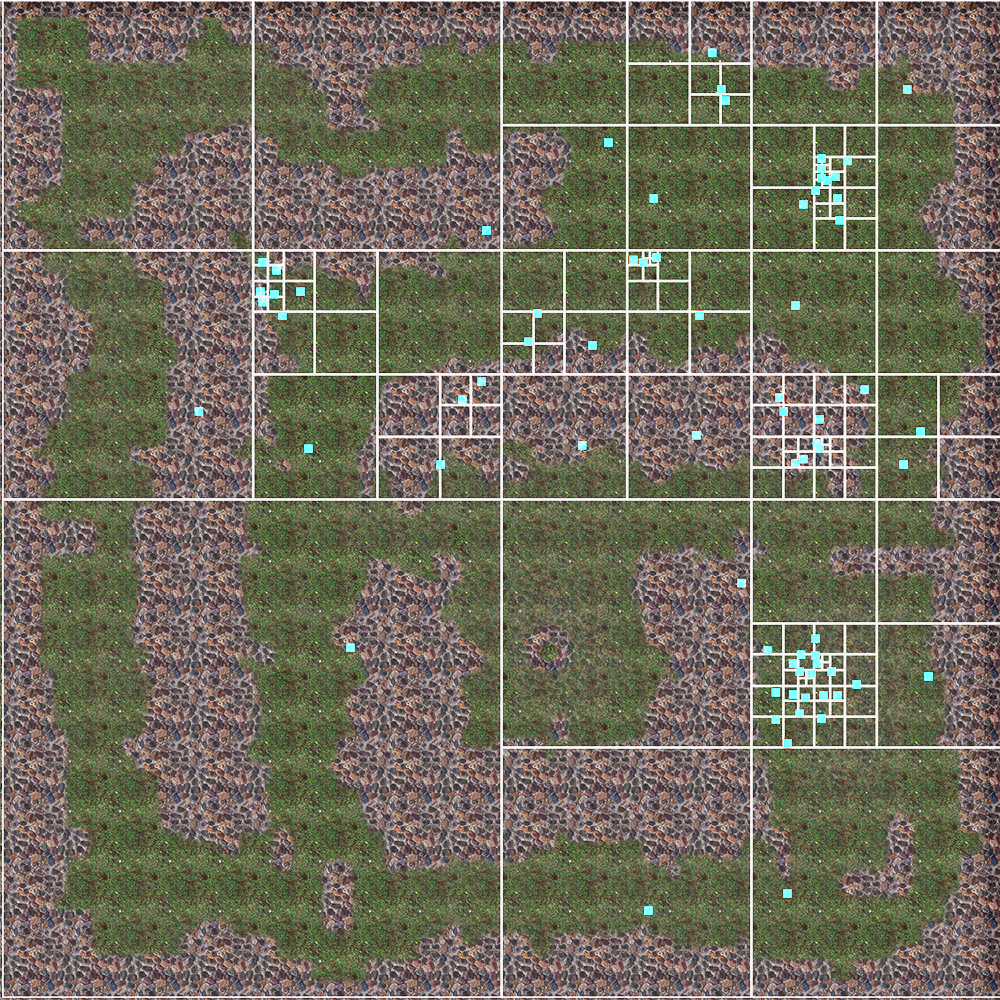
\includegraphics[scale=0.22]{kepek/quadtree.png}
\caption{A pálya felosztása a rajta lévő objektumok alapján}
\label{fig:quadtree}
\end{figure}

\subsection{A BSP fa}

Hasonlóan a négyes fához, ez is síkbeli felosztásra alkalmas. A BSP fa mindig két részre osztja a teret, viszont nem az adott térrész felénél, hanem úgy, hogy az objektumok száma a két részben közel egyenlő legyen. Az osztás irányát a fa minden mélységi szintjén változtatja, egyszer vízszintes, egyszer függőleges a vágás. Az adott objektumig úgy jutunk el, hogy mindig kiválasztjuk, hogy az éppen vizsgált térrészben az osztás bal, vagy jobb oldalán van. Kilépési feltételnek, szintén a négyes fához hasonlóan, megadhatjuk a fa maximális mélységét, illetve az adott cellában szereplő maximális objektumszámot.

\subsection{Optimalizálási módszer kiválasztása}

A saját játékom készítése során a négyes fát alkalmaztam, hogy optimalizáljam az erőforrások felhasználását a fölösleges számítások mellőzésével, de ez a módszer felhasználható még akár egy raktárépület területének felosztására, hogy a keresést optimalizáljuk, így kevesebb időt vegyen igénybe.

Azért a négyes fa alkalmazására esett a választás, mert ezt egyszerűbb volt implementálni, és a térrész magassága eleve limitált, így a $z$ összetevőnek kisebb a jelentősége.

\subsection{Program: Négyes fa}

Megvalósítás során meg kell adnunk a gyökér csomópontot, ami a teljes, felosztani kívánt területet takarja. Egy csomópont $x$ és $y$ pozíciót, $x$ és $y$ hosszt, 4 darab gyerek node-ot (ha nincs, akkor az adott node értéke $nullptr$), illetve egy pont tömböt tartalmaz.

Meg kell adnunk az objektumok helyét, amelyeket figyelembe véve történik meg a felosztás. Ha az objektumok száma a meghatározott értéknél nagyobb, az adott node gyerek node-jai meghatározásra kerülnek. Ez az egész folyamat egy rekurzív algoritmus. Gyerek node területének meghatározásánál, mivel a területet 4 felé osztjuk, adott, hogy mindkét oldalát feleznünk kell. A for ciklusban is a terület 4 felé osztása miatt megy az i 4-ig. 

\begin{algorithm}[H]
 \KwData{node; pontok\;}
 \KwResult{A teljes terület összes része}
  \If{pontok > küszöbérték}{
   	\For{i := 0; i < 4; i++}{
   		Adott node gyerek node-jának[i] := új node;\\
   		Gyerek node területének meghatározása;\\
   		Algoritmus rekurzív hívása\;
   	}
   }
 \caption{Négyes fa területfelosztás}
\end{algorithm}

A program indítása után a felhasználó által megadott objektumok száma, a terület mérete, és az egy területben lévő maximális objektumszám megadása után elvégzi a felosztást. Eredményként ahogy \aref{fig:quad_demo}. ábrán is szerepel, láthatjuk a kialakult struktúrát.

\begin{figure}[h]
\centering
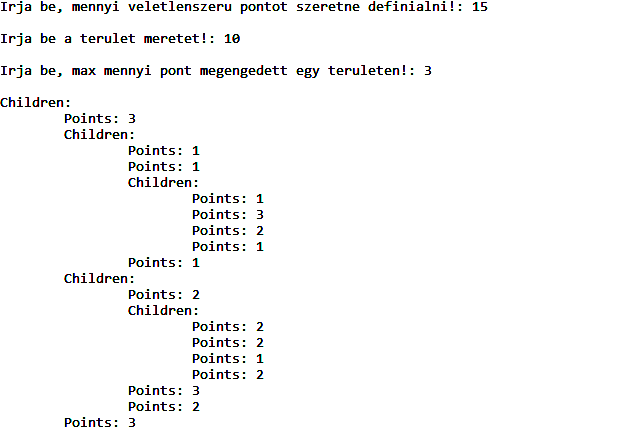
\includegraphics[scale=0.65]{kepek/quadtree_demo.png}
\caption{A négyes fa felbontással kialakult struktúra}
\label{fig:quad_demo}
\end{figure}

\Chapter{Útvonalkeresés}
\label{Chap:utvonalkereses}

A fejezet az útvonalkeresésnél alkalmazott módszereket mutatja be.

\Section{A waypoint-ok fogalma és jellemzői}

A waypoint a tér egy meghatározott pontja, amely nem látható a játékos számára. A mesterséges intelligencia ezeket használja fel az ellenfelek mozgási útvonalainak meghatározásához. Azért van rájuk szükség, mert a pályán különféle terepakadályok vannak (például falak), különböző játékelemek, amiken nem lehet átmenni, és ezekkel a pontokkal egyértelműen meg lehet határozni a bejárható helyeket.

A waypoint-okhoz rendelhetünk különféle többletinformációkat. Ilyenek lehetnek például, hogy az adott pontban a gépi játékosnak meg kell állnia, le kell guggolnia.

\Section{A waypoint-hoz tartozó adatok}

A waypoint-ok pozícióját két dimenziós Descartes koordináta rendszerben $(x, y)$ koordinátákkal adhatjuk meg. Annak ellenére, hogy térben vagyunk, nincs szükség $z$ koordinátára, mert a talaj magassága külön kezelendő, mivel az hatással lesz az ellenfelek viselkedésére. Ennek köszönhetően mindig az adott pálya talajmagasságához tud igazodni, nem szükséges azt külön megadni.

Fontos, hogy a waypoint-nak legyen egy típusa, amely meghatározza, hogy az adott pont milyen szerepet játszik. Ennek segítségével ki lehet számolni, hogy a játékban szereplő karakterek hova mehetnek.

\Section{Útvonalkeresés waypoint-ok alapján}

Tegyük fel, hogy a gép létrehoz egy ellenfelet egy véletlenszerű pozícióba. (Ezt a szakzsargonban \textit{spawn}-olásnak hívják.) Az ellenfeleknek az a fő feladatuk, hogy a lehető legrövidebb útvonalon eljussanak a játékoshoz, és megtámadják azt. 

Az útvonalkeresés folyamata a következő fő lépésekből épül fel:
\begin{itemize}
\item A waypoint-ok közül megkeressük az adott karakterhez vagy objektumhoz legközelebbit. Először ezt a pontot kell megközelíteni.
\item A waypoint-ok közül meghatározzuk a célponthoz legközelebbit, ez lesz majd a célpont.
\item A pont adott, kis sugarú környezetét elérve A*-algoritmus segítségével meghatározzuk a legrövidebb útvonalat.
\item A célpontot elérve már csak az adott karakterhez vagy objektumhoz kell egyenes úton eljutni.
\end{itemize}

\begin{algorithm}[H]
  \KwData{ \\
    $S \in \mathbb{R}^2$, a kezdőpont, aktuális pozíció \\
    $W = \{w_i | w_i \in \mathbb{R}^2\}$, a waypoint-ok halmaza
  }
  \KwResult{ \\
    $T \in \mathbb{R}^2$, az elérendő pont,
  }
  $\displaystyle T = \min_{||w_i - S||_2} w_i$
  \caption{A legközelebbi pont megkeresése}
\end{algorithm} 

\Section{Az A*-algoritmus}

Ezt az algoritmust a hatékonysága miatt gyakran használják gráfokban való legrövidebb útvonalak kereséséhez. Bemenetként a gráf két pontját adjuk meg, eredményül pedig az ezek között lévő legrövidebb útvonalat várjuk.

A gyakorlati problémák jelentős részében nem közvetlenül egy gráf áll a rendelkezésünkre. Ahhoz, hogy az A*-algoritmust mégis használni tudjuk, a bejárandó területet (amelyben a legrövidebb útvonalat keressük) egy ráccsal közelíthetjük. Ez a rácsos kialakítás több szempontból is előnyös. A pontok minden esetben egymástól egyenlő távolságra helyezkednek el, így ezeket nem kell számolni. Továbbá ha csak a bejárható helyekre helyeznénk pontokat, külön olyan algoritmusra lenne szükség, amely meghatározza azt, hogy melyik pontból melyikbe haladhatunk. A gráf összes csomópontjának és élének a tárolására szükség lenne, amely indokolatlanul sok adat kezelését jelentené. Jelen esetben egy egyenközű rácsot alkalmazva a kereséshez használt gráfhoz, elegendő csak megadni a rácspontokban, hogy az adott pont bejárható vagy nem \cite{Astar}.

Négyzetrács esetében eldöntendő kérdés, hogy az átlók mentén haladhatunk-e. Jelen esetben az tűnt megfelelőbbnek, hogy az átlók mentén is haladhatunk, ugyanis a játéktéren nem csak egymásra párhuzamos, és merőleges falak vannak, a domborzat lehet bármilyen elrendezésű.

Az algoritmus végrehajtásához listát kell vezetni azon pontokról amiket még nem jártunk be, illetve azokról is, amelyeket bejártunk, ezeket hívjuk nyitott (Open) illetve zárt (Closed) csomópont listáknak. A nyitott csomópontok listája az, amelyek vizsgálatára még a későbbiekben szükség lehet, a zárt csomópont lista pedig a már vizsgált pontok halmaza \cite{Astar2}.

A csomópontokhoz tárolni kell az addig bejárt távolságot, illetve le kell tárolni egy prioritás változót is, amiben az eddig megtett út, és a még hátralevő út távolságainak összege található. Fontos ugyanis az algoritmus működése szempontjából az eddig megtett, és a hátralévő út, mert ezekből az adatokból számolja ki egy adott pont prioritását (a kezdőponttól való távolságának és a célponttól való távolságának összegét), és így dönti el milyen pontokat részesítsen előnyben. A prioritás minél kisebb érték, annál jobb, tehát arra kell tovább indulni \cite{Astar3}.

\Section{Program: Útvonalkeresés A*-algoritmussal}

Az \texttt{Útvonalkeresés} nevű program célja, hogy bemutassa az A*-algoritmus egy lehetséges alkalmazását, amely felhasználható egyéb területeken is. Áruszállítás, vagy például mobil robotok útvonatltervezése esetén meghatározhatjuk a legrövidebb útvonalat $A$-tól $B$ pontig, akár mozgó $B$ pont esetén is \cite{mobile}.

A program a játéktér alapját képző domborzatot egy képből olvassa be. Ez a magasságmező, ahol egy adott pont magasságát a világossága határozza meg, minél világosabb, annál magasabb pontot jelent a domborzaton, így 256 különböző magasság lehetséges, amely az aktuális változathoz megfelelő felbontásnak bizonyult. 

A játékteret úgy érdemes kialakítani, hogy jelentős része (körülbelül 90\%) bejárható legyen.

A magasságmezőhöz tartozó kép felbontása $384 \times 384$ pixel, amely a térkép megfelelő részletességű megjelenítése miatt ennyi. Ez egy olyan felbontás, amely alatt már nagyon látszik a geometria gyenge részletessége a jelenlegi méret mellett, viszont a nagyobb felbontás már csak nagyon kis mértékben befolyásolná a kinézetet, ellenben növelné az erőforrásigényt. 

A waypoint-ok meghatározására több lehetőség is van. Az egyik lehetőség, ha minden pixelhez rendelünk egy pontot. Ez olyan szempontból lehet előny, hogy pontosabban meg van határozva az összes pont amelyre léphet az ellenfél. Hátránya viszont, hogy ez nagyon sok számításigény, és fölösleges is minden pixelre egy waypoint.

A másik lehetőség, ha 8 pixelenként határozunk meg egy waypoint-ot, ami 48x48-as felbontást eredményez. Azért pont erre az értékre esett a választásom, mert ez nagyban gyorsítja a számításokat, viszont még nem megy a bejárható területek rovására, megfelelően pontos. Ez kevesebb memória igényt jelent, és mivel kevesebb adattal is kell számolni, kevésbé terheli a processzort is. Ez látható \aref{fig:diagram_utvonal} ábrán.

\begin{figure}[h]
\centering
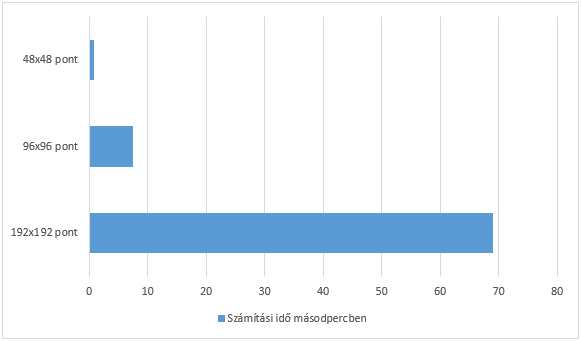
\includegraphics[scale=0.9]{kepek/utvonal_szamitas_diagram_waypointokra.png}
\caption{Számításigény a felbontás és idő(mp) függvényében}
\label{fig:diagram_utvonal}
\end{figure}

Első lépésként, létre kell hozni a waypoint hálót, amelyen a mesterséges intelligencia végig fog menni, elkerülvén hogy átmenjen a tereptárgyakon, falakon. Ezek a pontok 8 pixelenként, függetlenül az adott pixel színétől meghatározásra kerülnek, viszont a típusa az adott pixel színének megfelelően lesz beállítva. Ahogy \aref{fig:kuszobertek}-as ábrán is látható, a például egy pont színéből 50-nél nagyobb érték jön ki, akkor a pont típusa zártra állítódik, így ebbe az irányba nem lesz lehetséges a továbbhaladás. \Aref{fig:mi_printscreen}. képen feketével a falak, zölddel a kezdőpont, pirossal a célpont, fehérrel az útvonal van jelölve.

\begin{figure}[h]
\centering
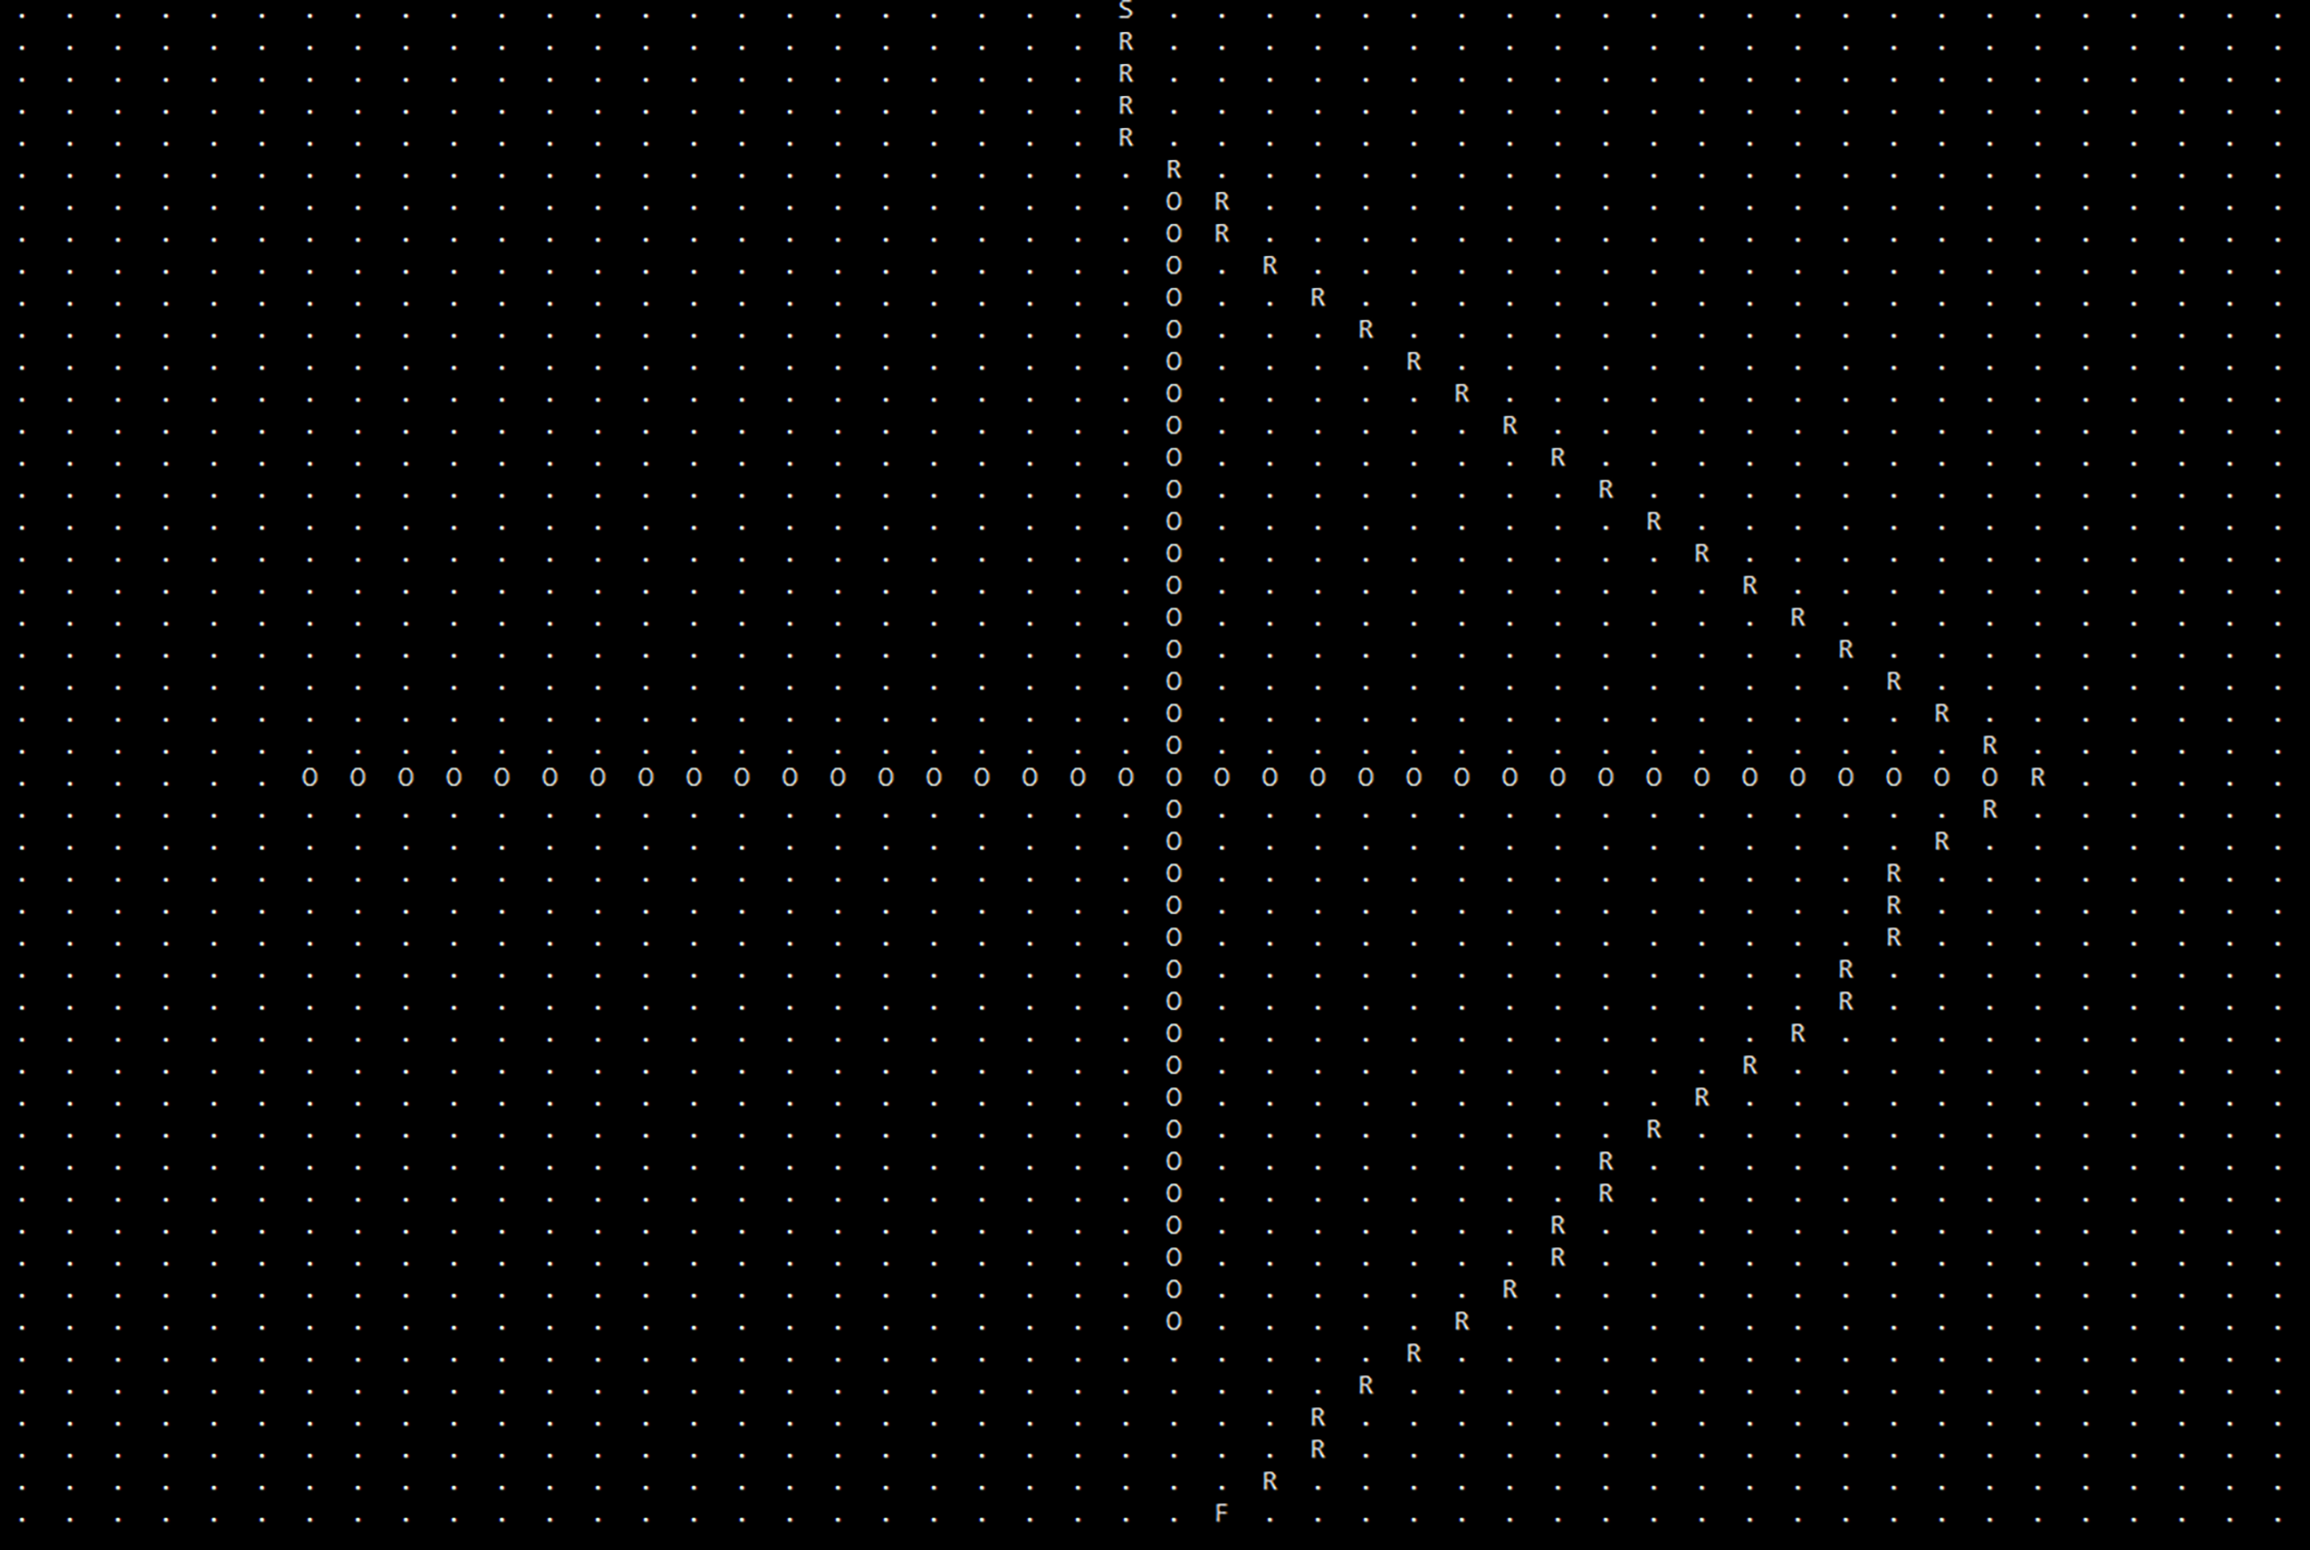
\includegraphics[scale=0.48]{kepek/mi_printscreen.png}
\caption{Útvonal meghatározó algoritmus működése}
\label{fig:mi_printscreen}
\end{figure}

A példaprogramban még csak statikusan vannak megadva a falak, de mint ahogy fentebb olvasható, a játékon belül a beolvasott magasságmező pontbeli értékei határozzák meg azt. Erre azért van szükség, mert így lehet megoldani azt, hogy a mesterséges intelligencia alkalmazkodjon a környezetéhez. Ha a pályától függetlenül, statikusan lenne az összes waypoint típusa meghatározva, akkor ha a játékos más pályát rajzol, a pontok típusai nem illeszkednének az elrendezésre. Ezt a módszert alkalmazva, meg lehet adni, hogy egy bizonyos magasságnál csak másszon, vagy ugorjon, vagy bármilyen más tevékenységet végezzen. Ez egy fontos tulajdonsága a játéknak, mert azt úgy terveztem, hogy a felhasználó tetszőleges raszteres rajzprogram segítségével elkészíthesse a térképet, ne legyen hozzá szükség speciális szerkesztőeszközre. A program a bejárható teret ebből képes közvetlenül meghatározni, be tudja állítani, hogy a falakon a játékos ne tudjon átmenni, a meredek lejtőkről visszacsússzon.

\begin{figure}[h]
\centering
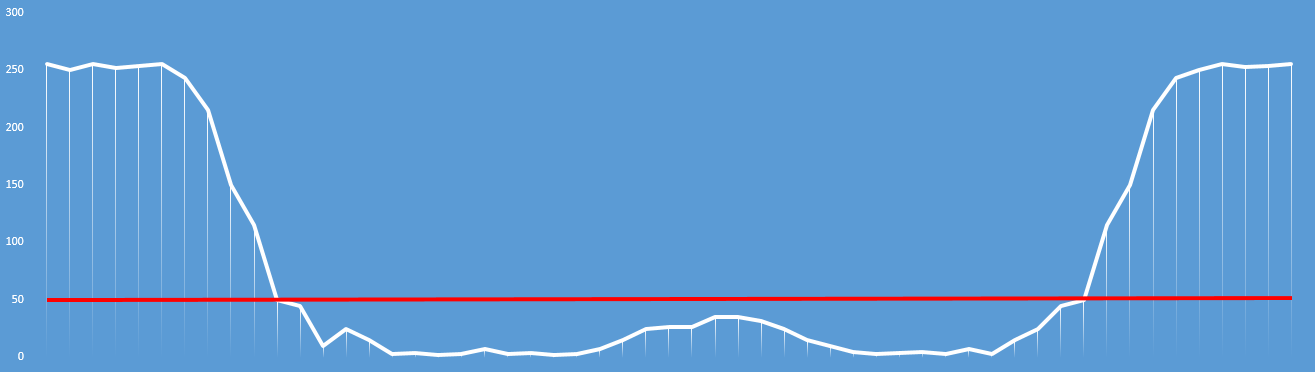
\includegraphics[scale=0.44]{kepek/magassagmezo_kuszobertek_diagram.png}
\caption{Küszöbérték a még bejárható terület meghatározásához}
\label{fig:kuszobertek}
\end{figure}

De a küszöbérték megadása nem mindig elegendő, ugyanis lehetnek olyan helyek a pályán, amelyek fal magasságúak, de bejárhatók, mert alacsony meredekségű emelkedő vezet fel oda. Ezt a problémát gradiens számítással lehet megoldani, ezzel van megoldva az is, hogy a játékos ne tudjon kimenni a játéktérből. Ahol túl nagy a meredekség, ott a waypoint típusát nem bejárhatóra kell állítani.

\newpage
A pontok típusának a pálya alapján legenerálása után, az A*-algoritmus segítségével meghatározza a játék a legrövidebb útvonalat a cél waypointig, természetesen a pontok típusait figyelembe véve. Ezt másodpercenként legalább 5x újra kell számolni, ugyanis a játékos mozog, és a cél waypoint mindig a játékoshoz legközelebb eső pont, ami ezzel együtt változik.

\Chapter{Animáció}
\label{Chap:animacio}

A fejezet a játékokban alkalmazott animációs módszereket, illetve azok megvalósítási módját mutatja be.

\section{Kulcsképkocka alapú animáció}

Kulcsképkocka alapú mozgatást több területen használnak, például filmek készítésénél vagy játékok fejlesztésénél. Bármilyen célra is használjuk, az elv nem változik. Meg kell adnunk olyan pontokat, amelyeket szeretnénk ha az adott tárgy, vagy objektum áthaladna. Ezzel egy előre meghatározott mozgási útvonalat adunk meg. Az egyszerűbb animációknál egy alapállapot és egy végállapot van megadva, ilyen lehet egy redőny leengedése és felhúzása, ajtó vagy kapu kinyitása, becsukása. Ilyen jellegű, alap szintű animációknál, például ha egy redőnyt le akarunk engedni, annyi a dolgunk hogy megadjuk a kezdő és végpontot, majd idő paraméter szerint interpolálni. Ahogy az \aref{fig:keyframe} ábrán látható, ez a kulcsképkockák közötti mozgást eredményezi.

\begin{figure}[h]
\centering
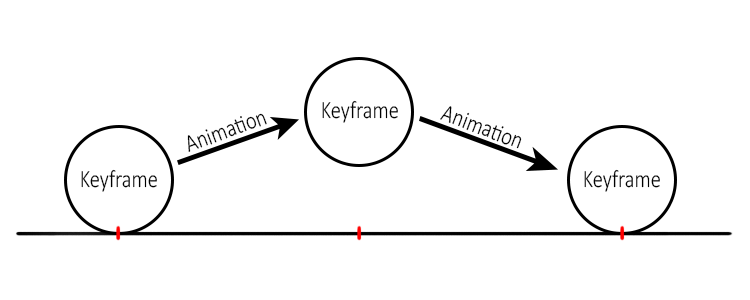
\includegraphics[scale=0.5]{kepek/keyframe_anim.png}
\caption{Kulcsképkocka alapú animáció}
\label{fig:keyframe}
\end{figure}

A vertex alapú animációt a 3D játékfejlesztésben karakterek mozgatásához a 2000-es évek elejéig használták. Megvalósítása egyszerűbb, viszont sok memóriát igényel a tárolása, és nem eredményez olyan természetes mozgást általában, mint a csontváz alapú animáció. Ezt a technológiát többek között a Quake 1, 2 és 3 alkalmazta.

\subsection{Az md2-es formátum}

% TODO: GL\_TRIANGLE\_FAN belelóg a margóba!

Az md2-es modelltárolási formátumot az \textit{idSoftware} fejlesztette ki 1997-ben a Quake 2 nevű játékához. A formátum kulcsképkocka animációk tárolására alkalmas. Tartalmazza az adott modell geometriáit, és a képkockánkénti animációkat. A fájl adatai olyan struktúrában helyezkednek el, hogy könnyedén kirajzoltatható legyen a \texttt{GL\_TRIANGLE\_FAN} és \texttt{GL\_TRIANGLE\_STRIP} OpenGL függvényekkel. A formátum két fő részből áll: fejlécből és adatrészből. A fájl nem tartalmazza a modellek textúráját.

A fejléc egy struktúra, amely a fájl elején kezdődik, és tartalmazza az összes, feldolgozás szempontjából lényeges információt a fájl egészéről. Ilyen például a textúra szélessége, magassága, egy képkocka mérete, képkockák száma.

\section{Csontváz alapú animáció}

A legtöbb mai játék ezt a módszert alkalmazza karakterek mozgatásához. Az alapötlete az, hogy a mozgatható részeket hierarchiába szervezi. Az élőlények felépítése általában olyan, hogy ezzel a fajta animálási móddal egyszerűen modellezhetők. 

A csontváz alapú animáció kapcsolódási pontokból (\textit{joint}-okból) építkezik. Ember esetén például a kézfej kapcsolatban van az alkarral, az alkar a felkarral, ami pedig a test többi részével. Minden hajlási pont egy új kapcsolódási pontot jelent. Tehát ha az ember felkarját megmozdítjuk, mozdul vele a kezének a többi része is. Ezt szemlélteti \aref{fig:skeletal}. ábra.

\begin{figure}[h]
\centering
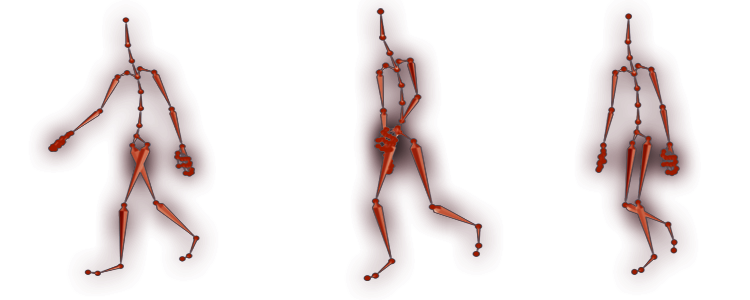
\includegraphics[scale=0.5]{kepek/skeletal_anim.png}
\caption[]{Testrészek hierarchikus kapcsolódási pontjai emberen\footnotemark}
\label{fig:skeletal}
\end{figure}

\footnotetext{forrás: https://www.openflipper.org/media/plugin\_images/skeletalAnimation.png}

Szerencsére a módszer nem csak élőlények modellezésére alkalmazható hatékonyan. A naprendszerünk szintén modellezhető ilyen módon. Vannak a naprendszerünk bolygói, amelyek a tengelyük, és a központi csillag, a Nap körül is forognak.

Előnye, hogy könnyen létre lehet így hozni dinamikus animációkat, mivel az összes karakter csontjait lehet forgatni, mozgatni, továbbá megkönnyíti a bonyolultabb animációk elkészítését. Hátránya viszont, hogy komplexebbek, így több processzoridőt igényelnek.

\subsection{Program: Animáció}

Ennek a programnak az a célja, hogy bemutasson egy animációs módszert, amelyet bárki fel tud használni karakteranimációhoz játékfejlesztésnél. Az animációt megvalósító algoritmus hasznos lehet még egy automatizált gyártósor robotkarjainak mozgatásához is olyan esetekben, amikor például két vagy több karnak mindig egy adott szög tartása mellett, összehangolva kell mozogniuk. A \texttt{Character} osztályban az összes mozgatással és azok pontos megjelenítésével kapcsolatos számítások találhatók. Az \texttt{Action} az állapotok kezeléséért, a \texttt{ModelLoader} és a \texttt{VboDrawer} a modellek (testrészek) betöltéséért, kirajzolásáért felelős, amelyeket a \texttt{MainGame} osztály fog össze. A konkrét felépítés \aref{fig:anim_uml} ábrán látható.

\begin{figure}[h]
\centering
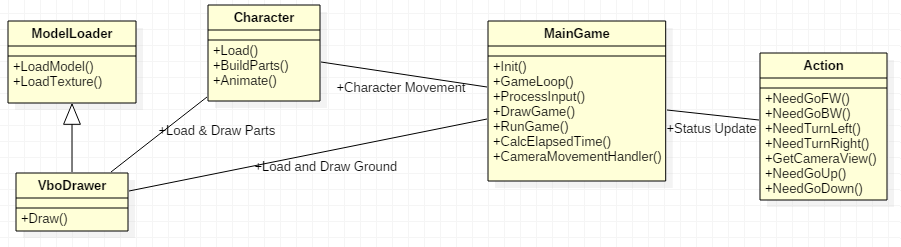
\includegraphics[scale=0.6]{kepek/animation_uml.png}
\caption[]{Az animációt bemutató demó felépítése}
\label{fig:anim_uml}
\end{figure}

\Aref{fig:anim_demo} ábrán látható, futó programban egy egyszerű robotot tudunk irányítani, illetve ha a kamerát szabad mozgás módba váltjuk, meg tudjuk tekinteni a testrészek hierarchikus mozgását több szögből is. A robot részei több .obj kiterjesztésű modellből vannak betöltve, amelyek azért vannak külön modellbe tárolva, hogy egymástól függetlenül tudjuk őket mozgatni, ne csak egyben a teljes robotot. A törzshöz csatlakozik a fej, a két kéz, és a két láb. Utóbbi kettő mindig 60 fokos szögkülönbséggel rendelkezik, és ha elérik a maximális, előre megadott kitérési értéket, a mozgás iránya megfordul. Az elérni kívánt mozgásmechanika implementálása után, meg kell adnunk a testrészek pozícióját. A \texttt{Character} oszályban lévő \textsl{BuildParts()} függvény a \texttt{ModelLoader} és a \texttt{VboDrawer} által betöltött és kirajzolt részek megfelelő pozícióba való elhelyezéséért felel, hogy azok egy egész robottá álljanak össze.

Járás közben az adott karakter előre is halad, illetve minimálisan fel és lefelé is mozog a járásból adódóan, és a testrészek fix szögben való mozgatásán kívül definiálnunk kell ezeket is. Figyelni kell, és számításba kell venni azt a jelenséget is, hogy járás közben egy élő ember  földre leért lába fix, azzal lendíti előre magát, így a láb végéhez képest kell megadnunk a hierarchiában feljebb lévő testrészek mozgását is, ezt nevezzük inverz kinematikának. Az előre és a fel-le irányba való mozgást a következő összefüggéssel írhatjuk fel:
$$
\Delta f = \left|
d \cdot \sin(\alpha)
\right|, \quad u = d \cdot \cos(\alpha),
$$

ahol $\Delta f$ az időegység alatt megtett előre mozgásnak a mértéke (\textit{forward}), az $u$ pedig a karakter fel-le mozgásának animálásához szükséges érték (\textit{up}). A $d$ az egységnyi idő alatt megtett távolságot jelöli (\textit{distance}), az $\alpha$ pedig a jobbláb animálásánál figyelembe vett szög értéke.

Az animálásért felelős részek időfüggőek, ugyanis garantálni kell hogy a különböző teljesítményű gépeken ugyanolyan gyors legyen az animáció. A két kirajzolt képkocka közötti eltelt időt a \texttt{CalcElapsedTime} függvény számolja, amelynek a kimeneti értéke az $s = v \cdot t$ képlettel számolható, ahol $s$ a megtett út, $v$ a sebesség, $t$ pedig az eltelt idő. Minél több a másodpercenként megjelenített képkockák száma, annál kisebb a köztük eltelt idő, és a mozgást annál kisebb értékkel szorozza be, így minden esetben ugyanolyan gyorsan fog mozogni az objektumunk, csak az animáció folytonosságában lesz különbség.

\begin{figure}[h]
\centering
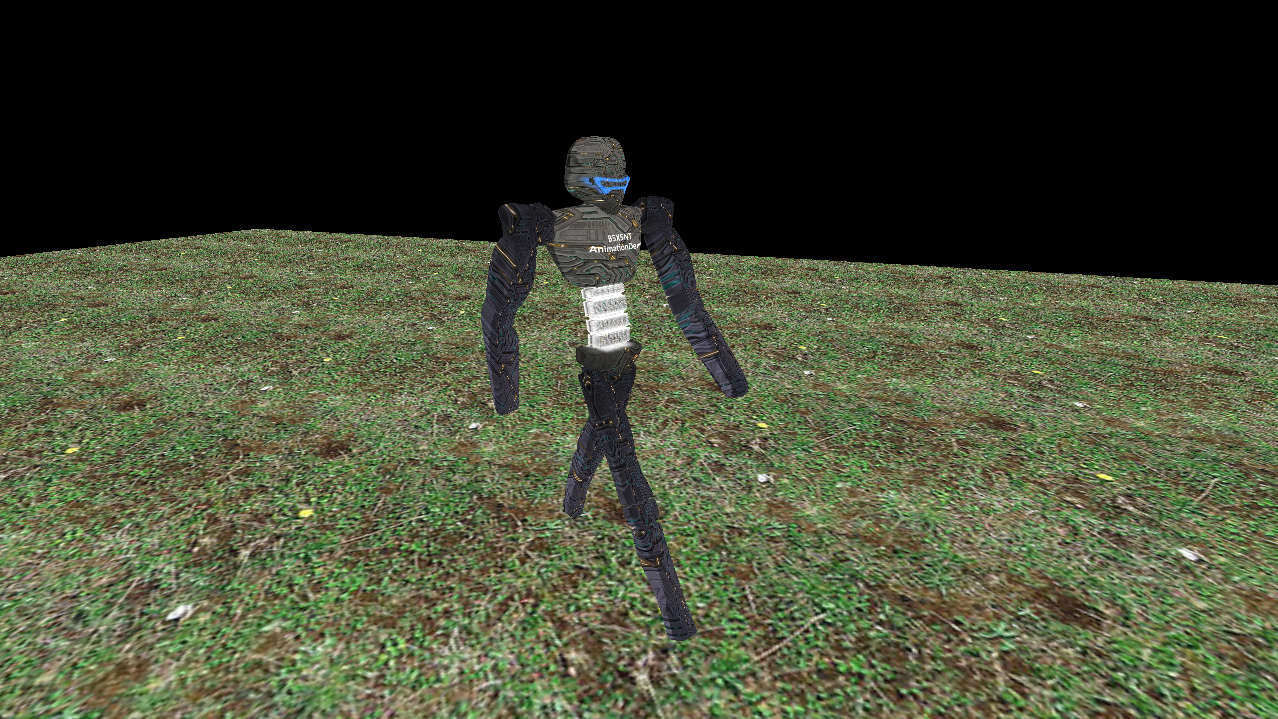
\includegraphics[scale=0.4]{kepek/animation_demo.png}
\caption[]{Pillanatkép az animációt bemutató demóból}
\label{fig:anim_demo}
\end{figure}

A kamera alapesetben a robot mögött van, és annak mozgását követi, amelyet szintén a felhasználó tud irányítani. Az animáció bármikor félbeszakítható, nem áll vissza az alapértelmezett állásba, hogy megtekinthető legyen a mozgás minden fázisa.

\section{Interpolációs módszerek}

% Interpoláció: https://hu.wikipedia.org/wiki/Interpol%C3%A1ci%C3%B3#Lagrange-interpol.C3.A1ci.C3.B3

Animációkészítés során többféle interpolációt használhatunk, ami azt jelenti, hogy ismert értékek alapján, a közbülső pontokra, vagyis nem ismert értékekre adunk közelítést.

Különféle interpolációs módszerek vannak. A választás közülük nyilván attól függ, hogy pontosan mit szeretnénk megvalósítani. Egyszerűbb esetekben még megfelelő a lineáris interpoláció, viszont általában túlságosan szögletes mozgást eredményez, ezért valamilyen simább görbével való útvonal közelítést érdemes használni.

\subsection{Lineáris interpoláció}

Ez a legegyszerűbb interpolációs módszer, minden pontot egy egyenessel kötünk össze. Nem összetett mozgásoknál ez megfelelő lehet, viszont ha több mozgás követi egymást rögtön, akkor darabos. Minden előre meghatározott pont, amit érinteni kell egy törést jelent, így komplexebb, sima mozgásokhoz nem alkalmas, ez látható \aref{fig:linear}. ábrán.

\begin{figure}[h]
\centering
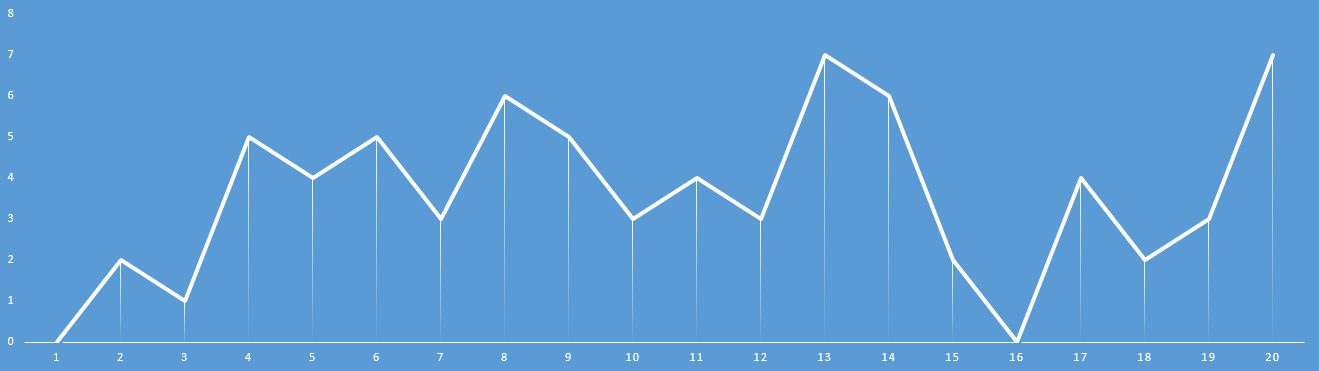
\includegraphics[scale=0.43]{kepek/linear_interpol.png}
\caption{Lineáris interpoláció}
\label{fig:linear}
\end{figure}

\subsection{Lagrange-interpoláció}

Mivel a függvény sima, deriváltja folyontos, sokkal életszerűbb megközelítést lehet elérni vele, mint a lineáris interpolációval. Viszont nagy hátránya, hogy egyes esetekben indokolatlanul nagy hullámzások jelenhetnek meg a kirajzolt függvényen, közvetlen egymás mellett lévő két pont között, ez látható \aref{fig:lagrange}-es ábrán. Így ez az interpoláció animációhoz nem minden esetben alkalmas.

\begin{figure}[h]
\centering
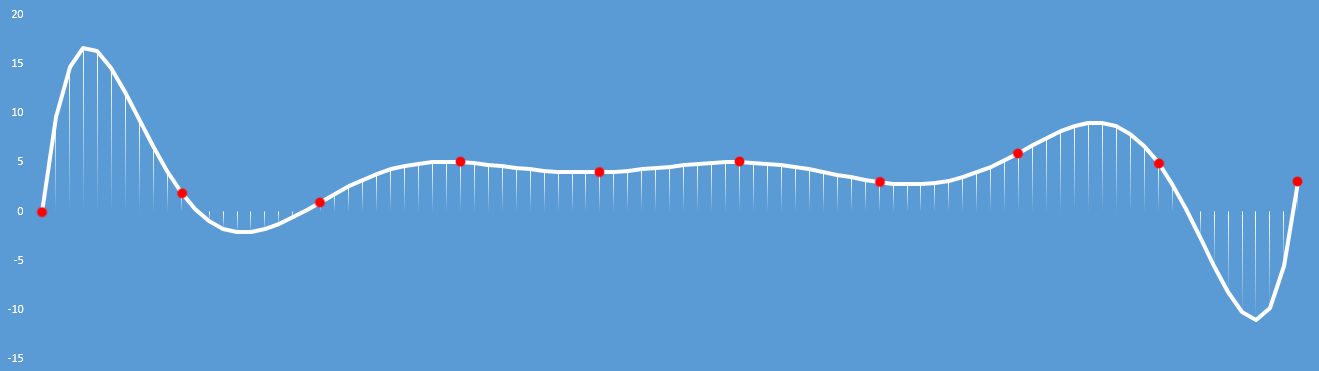
\includegraphics[scale=0.43]{kepek/non_linear_interpol.png}
\caption{Lagrange-interpoláció}
\label{fig:lagrange}
\end{figure}

\subsection{B-spline}

Komplexebb animációknál, mint például egy élőlény mozgása, ha nem szeretnénk darabos animációt, akkor a B-spline interpolációt is alkalmazhatjuk. Ez esetben a görbe lokálisan vezérelhető, és a lineáris interpolációval ellentétben nem töredezett, így ez a legalkalmasabb folyamatos animációra. A lokális vezérelhetőség adja az előnyét a Lagrange-interpolációval szemben, mert így nem lehetnek kiugró értékek a grafikus képében.

\subsection{Program: Lagrange Interpoláció}

A felhasználónak lehetősége van megadni, hogy hány darab pontot szeretne definiálni, majd a pontok konkrét $x$ és $y$ koordinátáit, amelyekhez a program kiszámolja az y koordinátát Lagrange-interpolációval. Ez a program azért készült, hogy bemutassa, hogyan működik ez a fajta interpolálás.
Adott két tömb, amelyek tartalmazzák a függvény megadott pontjainak x és y értékeit. A num a tömbök elemeinek számát, az input pedig a bevitt értéket takarja.

\begin{algorithm}[H]
 \KwData{x[]; y[]; num; input; s; t; eredmeny\;}
 \KwResult{Adott x-hez tartozó y koordináta}
\For{i := 0; i < num; i++}{
	s := 1, t := 1\;
	\For{j := 0; j < num; j++}{	
	\If{j != i}{
   		s := s * (input - x[j]);\\
		t := t * (x[i] - x[j])\;
   		}
	}
	eredmeny := eredmeny + ((s / t) * y[i])\;
 }
 \caption{Lagrange-interpoláció implementálása}
\end{algorithm} 

A függvény grafikus megjelenítése az OpenGL-el lett megvalósítva. Az ablak alapértelmezett felbontása 1280x720, amelyhez a bevitt értékeket a program felskálázza úgy, hogy a függvény még sehol sem lógjon ki az ablakból, de a lehető legnagyobb méretű legyen. A skálázás mértékét mind konzolban, mind grafikusan megjeleníti, utóbbit csak addig, míg a szorzó nagyobb mint 9. Ez alatt az osztás már olyan sűrű 1280x720-as felbontás mellett, hogy értelmetlen, és csúnya a grafikus kirajzolása. 
\newpage
A függvény kezdete a legkisebb, a vége pedig a legnagyobb $x$ értéknél van, a köztes részen pedig minden egész $x$-hez kiszámolja a hozzá tartozó $y$-t, majd azokat vonallal összeköti. A konzol eredményei \aref{fig:lagrange_imp}. ábrán, a grafikus megjelenítés pedig \aref{fig:lagrange_demo}. ábrán látható.

\begin{figure}[h]
\centering
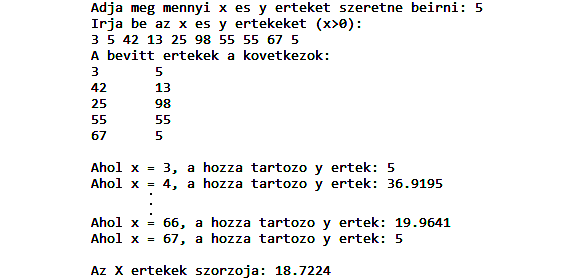
\includegraphics[scale=0.9]{kepek/lagrange_imp.png}
\caption{Lagrange-interpolációs demó}
\label{fig:lagrange_imp}
\end{figure}

\begin{figure}[h]
\centering
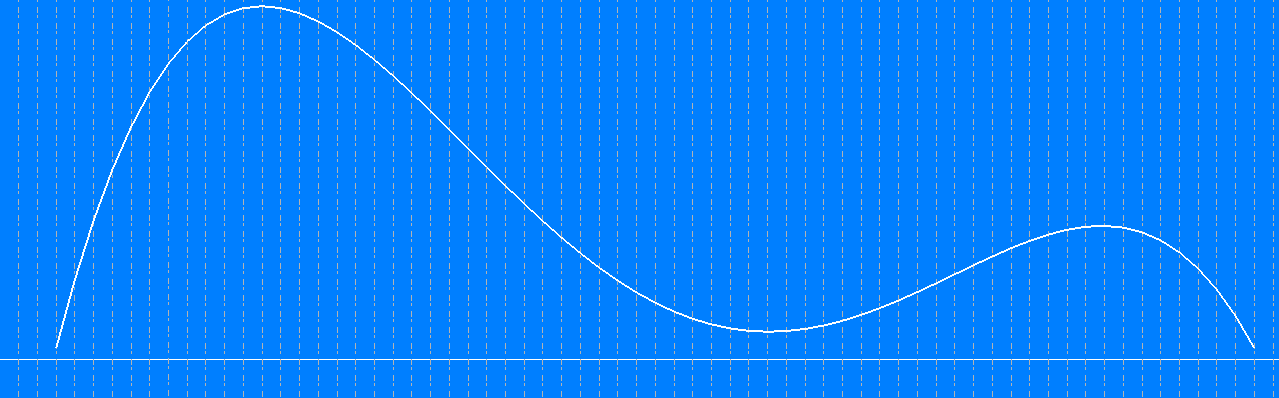
\includegraphics[scale=0.43]{kepek/lagrange_graphics.png}
\caption{Lagrange-interpolációs demó}
\label{fig:lagrange_demo}
\end{figure}


\Chapter{Ellenfelek viselkedésének modellezése}
\label{Chap:viselkedes}

%Ágens alapú viselkedés

%- Leírni, hogy milyen bemenetek és kimenetek szükségesek ahhoz, hogy az %ellenfelek viselkedését modellezzük.

%Klasszikus, állapotgép alapú modell bemutatása
%Véletlenszerű tényezők a játék érdekesebbé tételéhez

A mesterséges intelligencia útvonalkeresés részéről már szó volt a korábbiakban, viszont nagyon fontos, hogy az ellenfeleknek egyéb tulajdonságokat adjunk, ezzel érdekesebbé téve a játékot. Szüksége van minden ellenfélnek egy célra, ami alapjában véve az, hogy megtámadják a játékost, viszont bizonyos szituációkban ez megváltozik, így kapunk még élethűbb viselkedést. Ez a fejezet ezen elemek bemutatásáról szól.

\section{Viselkedés bemenetei és kimenetei}

Ahhoz hogy az ellenfelek viselkedését modellezzük, különböző bemenetekre és kimenetekre van szükség.

\subsection{Bemenetek}
Bemenetként az ellenfél szemszögéből számít a játékostól való távolság, az aktuális életerő, a lőszer mennyisége, hogy a játékos benne van-e a látótérben, illetve hogy egyedül kell-e neki szembeszállni a játékossal, vagy többen vannak. Ezek a bemenetek egymástól is függhetnek. Ha a játékostól való távolság kisebb, mint egy előre definiált érték, és nem egyedül vannak, akkor közelítsenek és támadjanak, viszont ha egyedül van, akkor próbáljon menekülni. Figyelembe veheti azt is, hogy milyen hatékony fegyver van a kezében, az életereje vagy lőszere egy előre definiált érték alatt van-e, és ezek függvényében támad, keres életerőt vagy lőszert. Az ilyen típusú adatok definiálásának legjobb módja, ha az ellenféltípusokhoz hozzárendelünk különböző tulajdonságokat, így kialakíthatjuk, hogy melyik miben jó, és miben rossz. Ezt nevezzük karakterisztikának.

\begin{figure}[h]
\centering
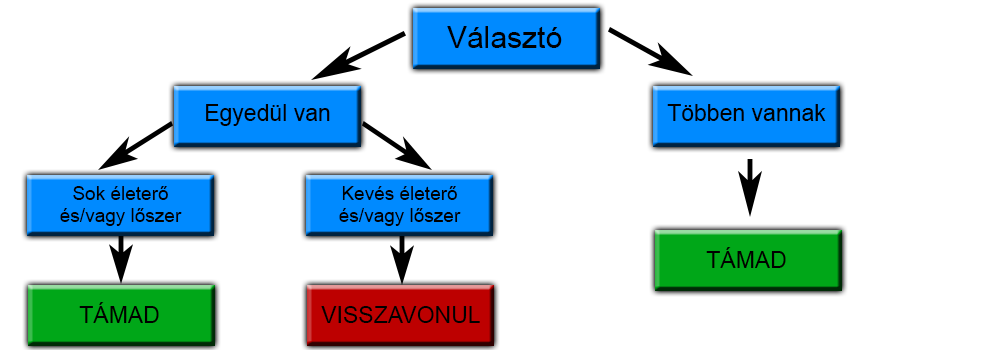
\includegraphics[scale=0.38]{kepek/viselkedes.png}
\caption{Az ellenfél egy lehetséges viselkedése}
\label{fig:behavior}
\end{figure}

\subsubsection{Adott ellenfél karakterisztikája}

\begin{tabular}{r|l}
Név & Az ellenfél neve. \\
Támadóképesség & Ellenfél képességei támadás közben.\\
&> 0.0 \& < 0.15 = Nem mozdul.\\
&>= 0.15 \& < 0.5 = Csak előre és hátra mozog.\\
&>= 0.5 \& < 1.0 = Körbe-körbe megy.\\
&> 0.6 \& < 1.0 = Véletlenszerű mozgás irányváltással.\\
&> 0.4 \& < 1.0 = Visszavonuláskor is fedezze magát lövéssel.\\
Agresszió & Az ellenfél agressziója.\\
Neme & Férfi, nő, vagy egyéb teremtmény\\
Célzóképesség & Fegyverenként különbözhet.\\
&> 0.0 \& < 0.9 = Az ellenfél mozgása hatással van a célzásra.\\
&> 0.4 \& <= 0.8 = Ellenfélmozgás követése.\\
&> 0.8 \& <= 1.0 = Várható felbukkanás helyének figyelése.\\
&> 0.6 \& <= 1.0 = Környezeti elemek felhasználása sebzésre.\\
Guggolás & Guggolás gyakorisága.\\
Ugrás & Ugrás gyakorisága.\\
Forgás & Forgás sebessége (reflex).\\
Reakcióidő & Miután meglát, mennyi idő telik el az első lövésig.\\
Lövéspontosság & 0 és 1 közötti érték, a lövés szórását adja meg.\\
Bosszú & Az ellenfél bosszúállósága.\\
\end{tabular}

\subsection{Kimenetek}

A bemeneti adatok alapján a program egy modulja kiértékeli az eseményeket, és annak kimeneti értékei határozzák meg a következményeket. Minden kimenet egy végrehajtható akciót jelöl (támadás, menekülés, életerő vagy lőszer töltés). A döntési fa az csak az állapotot határozza meg. Minden iterációban ki kell értékelni, és minden lehetséges esethez meg kell írni azt a kódrészt, ami az adott cselekvésfolyamatot elindítja. \Aref{fig:behavior}-es ábrán kékkel vannak jelölve a bemeneti paraméterek, zölddel és pirossal pedig azok következményei, vagyis a kimenetek.

\subsection{Program: Behavior Demo}

Ezen a program elkészítésével az volt a célom, hogy minél egyszerűbben, vizuálisan lehessen bemutatni az ellenfelek viselkedését. A termelésinformatikában ennek az algoritmusnak a segítségével különböző döntési tényezőket lehet definiálni, hogy a robot azoknak megfelelően cselekedjen. Jelen esetben a játékost fehér, az ellenfeleket piros, a biztonságos pontokat kék négyzet jelöli. A biztonságos pontok azok a helyek, ahova egy ellenfél vissza tud vonulni, ha a játékos megmozdul. Minden ellenfél a korábban leírtaknak megfelelően rendelkezik egy karakterisztikával, amely minden esetben két tulajdonságból áll, a sebességből, és a félelemfaktorból. Utóbbi azt határozza meg, hogy ha megmozdul a játékos, mekkora legyen az a sugár, amelybe ha egy biztonságos pont beleesik, visszavonuljon. Ha több pont esik az adott sugárba, akkor azok közül is a legközelebbit választja.

A félelemfaktor függ az ellenfél sebességétől is, tehát gyors ellenfél esetén csak alacsony értékeket, lassú ellenfél esetén pedig csak magas értékeket vehet fel, ezzel életszerűbbé teszi a viselkedést. A mintaprogram felépítése \aref{fig:behavior_uml} ábrán látható.

\begin{figure}[h]
\centering
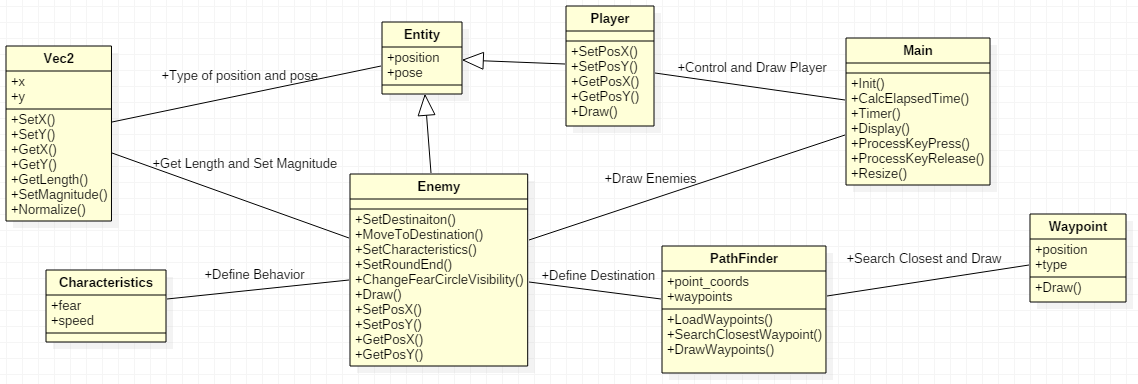
\includegraphics[scale=0.5]{kepek/behavior_uml.png}
\caption{A viselkedést bemutató program felépítése}
\label{fig:behavior_uml}
\end{figure}

\Aref{fig:behavior_settings} ábrán látható módon, az elindítás után minden ellenfélnek véletlenszerűen generál egy karakterisztikát, olyan módon, hogy a sebességet és a félelemfaktort beállítja egy adott értékre. A felhasználónak lehetősége van ezeket újragenerálni, illetve minden ellenfélnek a félelemfaktorát vizuálisan megjeleníteni, amely \aref{fig:behavior_demo} ábrán látható.

\begin{figure}[h]
\centering
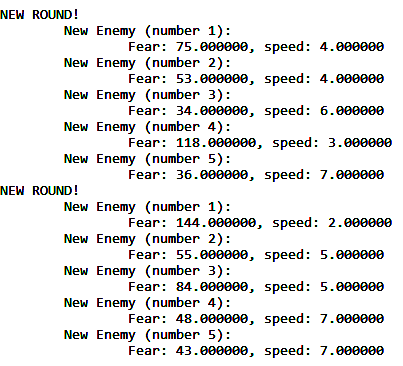
\includegraphics[scale=0.8]{kepek/anim_random_values.png}
\caption{Az ellenfelek félelemfaktora}
\label{fig:behavior_settings}
\end{figure}

\begin{figure}[h]
\centering
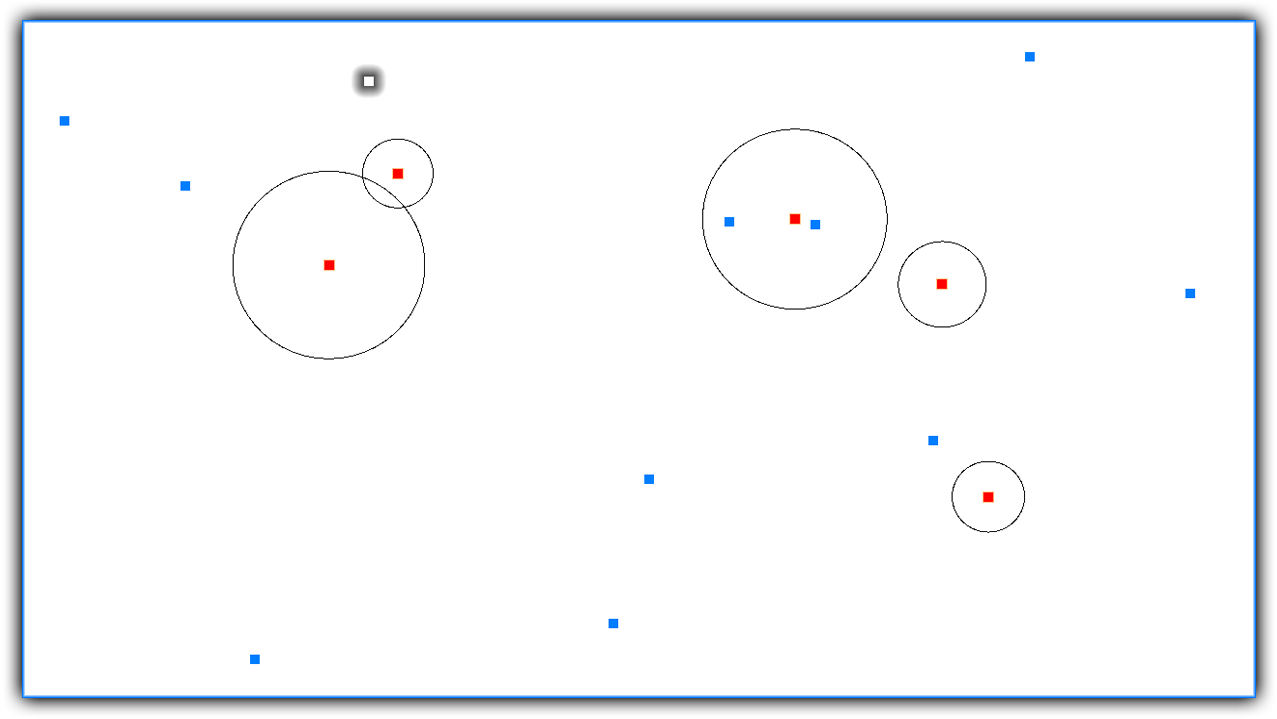
\includegraphics[scale=0.4]{kepek/behavior_demo.png}
\caption{Az ellenfelek félelemfaktora}
\label{fig:behavior_demo}
\end{figure}

\section{Véletlenszerű tényezők}

A játékban el vannak helyezve különböző használható elemek, amelyek kihatással vannak a játékmenetre. Viszont az, hogy annak milyen mértékben van hatása pozitív irányban, csak akkor derül ki, ha már felvettük azt. Különböző típusú elemek léteznek, amiket a mesterséges intelligencia által vezérelt ellenfelek is tudnak hasznosítani. A játéktéren találhatunk életerőre, lőszerre és csapda megjelenési idejére hatással levő elemeket.

\subsection{Konkrét megvalósítás}

Az életerő és a lőszer megvalósítás szempontjából egy egész (integer) típusú, a csapda megjelenési ideje pedig egy tört (float) szám. A felvehető elemek ezeket az értékeket módosítják különböző mértékben. Ezek egyikének megvalósítása \aref{fig:health} ábrán látható.

\begin{itemize}
\item Életerőt véletlenszerűen 10, 25 vagy 50\%-kal növelheti. 
\item Lőszerhez véletlenszerűen adhat 15, 30, vagy 50 darabot.
\item Csapda megjelenési idejét véletlenszerűen növelheti 25, 50 vagy 100\%-kal.
\end{itemize}

\begin{figure}[h]
\centering
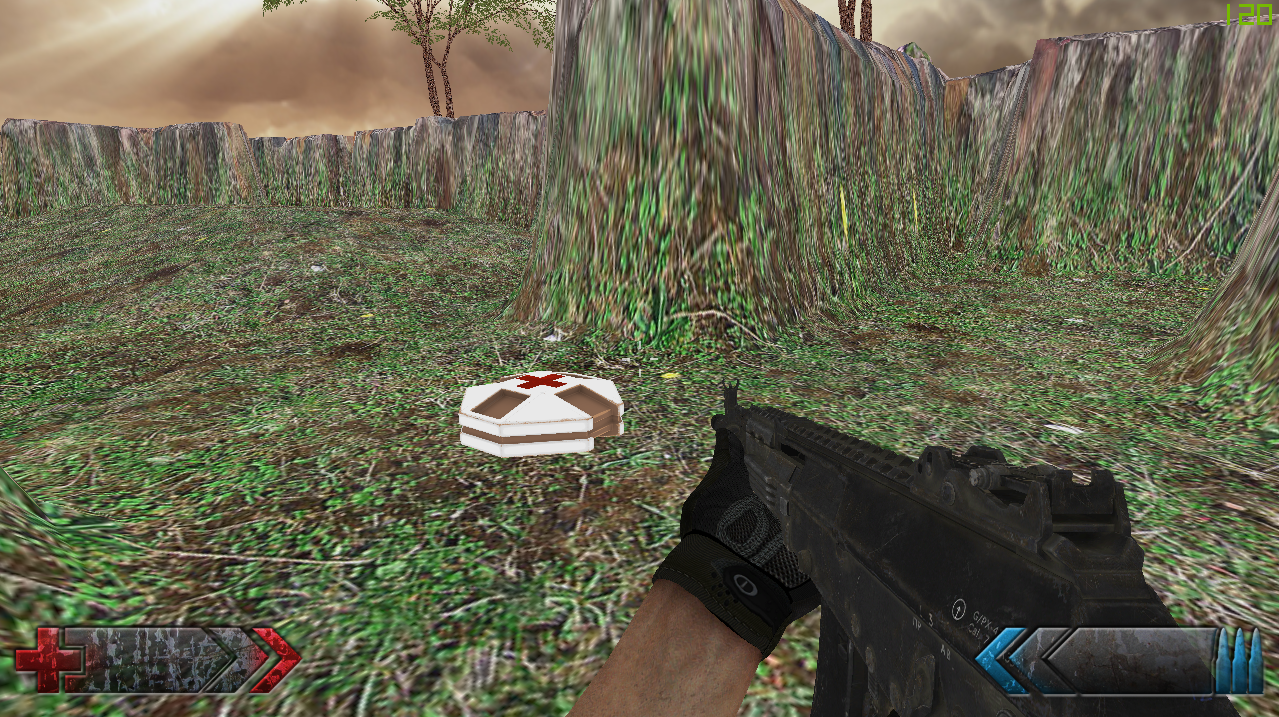
\includegraphics[scale=0.4]{kepek/health.png}
\caption{Egy felvehető elem a játékban}
\label{fig:health}
\end{figure}


\Chapter{Tesztek}
\label{Chap:tesztek}

%A játékmotor vizsgálata egy az egyben
%Review jellegű észrevételek
%Profilozás

Ez a fejezet az általam írt játékmotor, illetve az azzal megvalósított funkciók különböző megvalósításainak tesztjeiről szól. Különböző elemeket, különféle módszerrel lehet implementálni, többféleképp lehet optimalizálni, amelyek kirajzolási idejében különbségek vannak. Léteznek kisebb és nagyobb hatékonyságú algoritmusok a különböző problémák megoldására.

\section{Kirajzolási módszerek}

Alapvetően két fő kirajzolási módszer létezik az OpenGL-ben. Az egyik a régebbi glBegin-glEnd blokkos, a másik a modernebb Vertex Buffer Object-es (VBO). A kettő között a legfőbb különbség a gyorsaság. VBO-s megjelenítési mód esetén, mint ahogy a nevében is benne van, egy buffer-be (tárólóba) betöltjük az összes kirajzolni kívánt elemet, és azt egyben adjuk át a videokártyának, a legmegfelelőbb formátumban. Ez sokkal gyorsabb, mivel a régebbi egyesével adja át a pontokat kirajzolásra. \Aref{fig:old_fps}-es ábrán a régebbi, \aref{fig:vbo_fps}-es  ábrán pedig a VBO-s megjelenítési mód látható. Ugyanazoknak az objektumoknak a kirajzolása sokkal gyorsabb VBO-val, ez látható mindkét képen a bal felső sarokban. Sokkal jobb a hardver kihasználtsága is, és az FPS (képkocka/másodperc) is kicsivel több, mint 8x magasabb.

\begin{figure}[h]
\centering
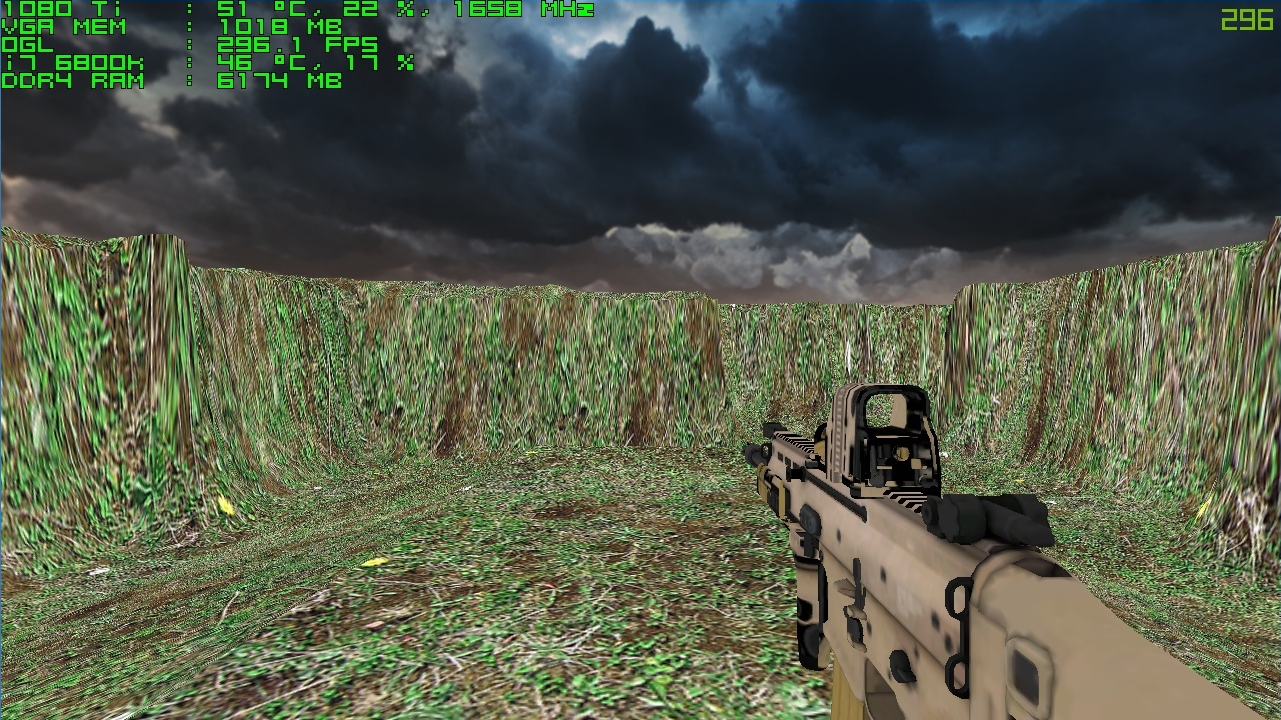
\includegraphics[scale=0.38]{kepek/old_method_fps.png}
\caption{A terep kirajzoltatása a régebbi módszerrel}
\label{fig:old_fps}
\end{figure}

\begin{figure}[h]
\centering
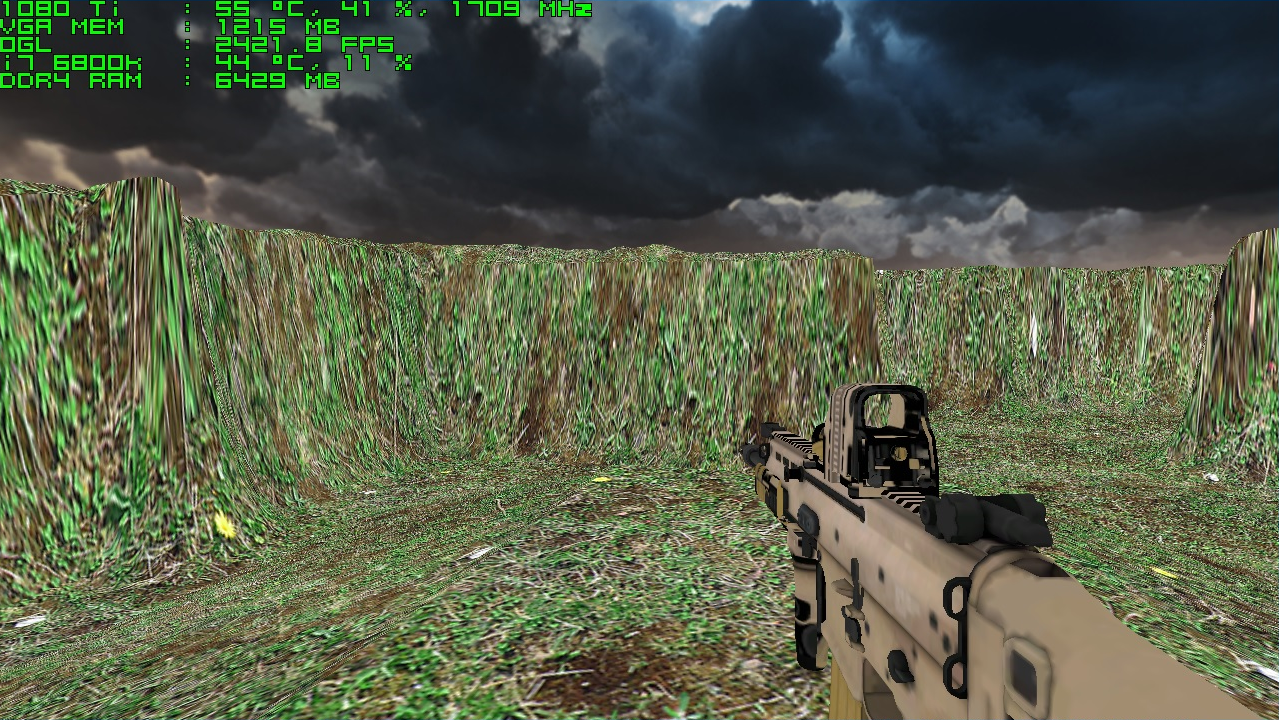
\includegraphics[scale=0.38]{kepek/vbo_method_fps.png}
\caption{A terep kirajzoltatása az újabb, VBO-s módszerrel}
\label{fig:vbo_fps}
\end{figure}

\section{Profilozás}

A játék egyes elemeinek betöltéséről, kirajzolásáról diagramok készültek. Minden ábrán, a függőleges tengelyen az adott objektum, vagy elem neve látható, a vízszintes tengelyen pedig az idő van feltüntetve milliszekundumban.

\Aref{fig:start_diag}-as ábra a játékindítás folyamatának időigényét részletezi, hogy az egyes elemek létrehozása, betöltése hogyan oszlik el a teljes időhöz képest. Mint látható, az időtartam nagy részét a képi elemek betöltése teszi ki, a további négy elem szinte elhanyagolható ilyen szempontból.

\begin{figure}[h]
\centering
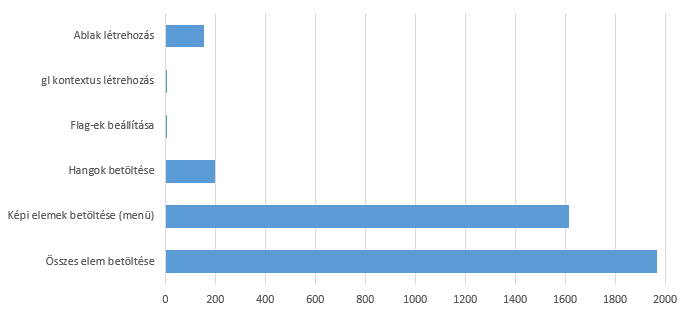
\includegraphics[scale=0.84]{kepek/start_diag.png}
\caption{Játékindítás teljes ideje a menübe való eljutásig}
\label{fig:start_diag}
\end{figure}

\Aref{fig:map_diag}-es ábrán a teljes játéktér betöltésének, illetve az egyes részek betöltésének ideje látható.

\begin{figure}[h]
\centering
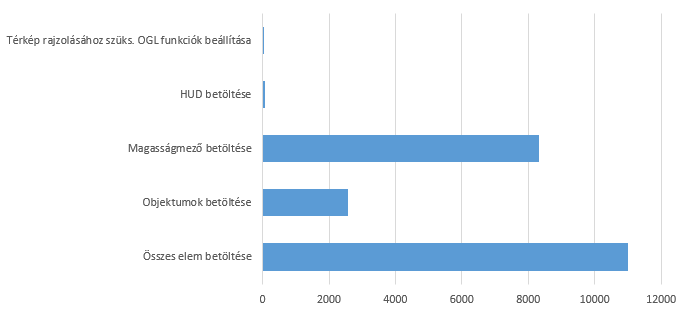
\includegraphics[scale=0.84]{kepek/map_load_diag.png}
\caption{A játéktér betöltésének ideje}
\label{fig:map_diag}
\end{figure}

Mivel a magasságmező betöltésének ideje nagyon kiugró, külön megvizsgáltam (\ref{fig:height_map_diag}-ös ábra), hogy azon belül melyik rész okozza ezt. Feltűnő, hogy a magas betöltési időt a textúra betöltése okozza, mert nagy a felbontása. Ezen javítani úgy lehet, hogy kisebb felbontású textúrát választunk, és azt többször helyezzük a magasságmezőre. Ha ezt a megoldást válasszuk, akkor a jelenleg is alkalmazott módszert, miszerint a pálya elrendezésének megfelelően rajzoljuk be a magas pontok textúráit, nem lehet megvalósítani, mivel a többszörös ismétlés miatt nem fog illeszkedni.
 
\begin{figure}[h]
\centering
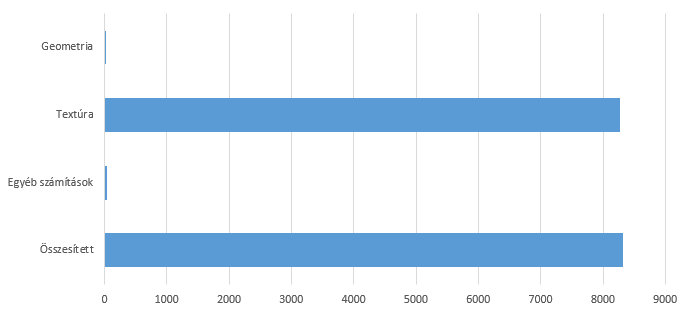
\includegraphics[scale=0.84]{kepek/height_map_load_diag.png}
\caption{A domborzat betöltésének ideje részletezve}
\label{fig:height_map_diag}
\end{figure}

\newpage
Végső soron megvizsgáltam, hogy egy képkocka elkészülése során, melyik játékkomponens megjelenítése vagy számítása hogyan oszlik el a teljes képkocka idejének elkészüléséhez képest. Ez fix 120 másodpercenkénti képkockaszám (FPS) mellett lett kiszámolva. Tudjuk, hogy 120FPS esetén a képkockák kirajzolása között eltelt időtartam 8,33ms, így elég volt csak a modellek, illetve a magasságmező kirajzolásának idejét mérni, a maradék értelemszerűen a további háttérszámításokat teszi ki.
A másik ok, ami miatt fix FPS-t választottam a méréshez, az a túl magas másodpercenkénti képkockaszám (átlag 2000FPS) korlátozás nélkül. Ilyen esetben a képkockák kirajzolása között eltelt időtartam annyira kicsi volt, hogy még milliszekundumban is mérhetetlen volt.

\begin{figure}[h]
\centering
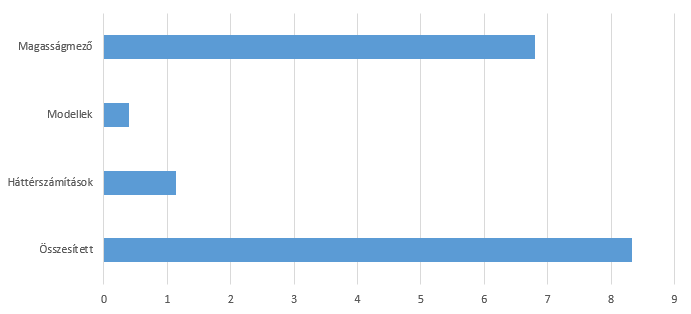
\includegraphics[scale=0.84]{kepek/frame_draw_diag.png}
\caption{Egy képkocka kirajzolása (120FPS esetén)}
\label{fig:frame_draw}
\end{figure}
\Chapter{Összegzés}
\label{Chap:osszegzes}

A dolgozatban olyan optimalizálási módszerek kerületek bemutatásra, amelyek nagyban csökkentik egy adott játék, (vagy általában egy alkalmazás) erőforrásigényét. A bemutatott eszközök gyakran szükségesek ahhoz, hogy egy komplex grafikus alkalmazás optimalizációját a fejlesztők el tudják végezni.

A játékfejlesztés egy nagyon időigényes munka, ugyanis az esetek jelentős részében szükség van a kód optimalizálására. E nélkül az alkalmazások nem lennének képesek a virtuális valóság valós idejű megjelenítésére, vagy csak jóval nagyobb hardverigény mellett. Egy mai modern játékot olyan hatalmas bejárható terület, valószerű fizika, illetve szép, szinte teljesen valósághű grafika jellemez, amely akár még fél évtizede is elképzelhetetlen lett volna.

A megjelenítéshez az OpenGL grafikus függvénykönyvár került felhasználásra. Ahhoz, hogy a megjelenítés sebessége elfogadható legyen, vertex buffer objektumok (VBO-k) használatára volt szükség.

A dolgozat bemutatja a négyes fákat és az oktális fákat, amelyek a nagy játéktérben való keresés optimalizálásában segítenek. A karakter ütközésvizsgálatának szempontjából a probléma annyival komplexebb, hogy ott mozgó karakterről van szó, amelynél az ütközésvizsgálatot a karakter több pontjára is el kell végeznünk.

A lövések esetében a találatok regisztrálását egy egyszerűsített geometriára szokták elvégezni. Ez szintén egy olyan optimalizálási módszer, ami ahhoz szükséges, hogy a játék futási ideje elfogadható legyen, még nagyobb méretű térképek esetében is.

Mivel egy modern játék esetében az egyik fő cél az, hogy minél valóságszerűbb legyen a játékmenet, ezért a karakterek mozgatására is kiemelt figyelmet kell fordítani. A dolgozat bemutatja az ezek mozgatásához gyakran használt csontváz alapú karakteranimálási módot és ehhez kapcsolódóan az elterjedt interpolációs görbéket.

\Chapter{Summary}

The thesis presents some of the well-known optimization methods, which are able to decrease the resource requirements of a computer game or an application. The mentioned methods are essential for developers for creating complex graphical applications.

The game development is a time consuming task, because we have to optimize the resulted source code for achieving acceptable performance. Without these steps, the applications were not able to render the frames of the virtual reality in real-time. The modern computer games have large, explorable areas, realistic physics and photorealistic graphics, which was unimaginable a half decade ago.

The application uses OpenGL for rendering. For the acceptable performance we have to use vertex buffer objects (VBO).

This work explains the concept and implementation of quadtrees and octrees, which makes the searching in large game space efficient. The collision detection of characters is much more complex, because the characters can move and they have more points.

In the case of bullets, the registration of the hits is usually applied to a simplified geometry. It is also an optimization method which necessary for real-time games in the case of large maps.

The realistic game mechanics is also one of the main goal of modern games. Therefore, we have to consider the details of character animations. This work presents the frequently used skeleton-based animation methods and the corresponding interpolation curves.


\begin{thebibliography}{x}
\addcontentsline{toc}{chapter}{\bibname}

\bibitem{Unreal}
Az Unreal motorról bővebben: https://en.wikipedia.org/wiki/Unreal\_Engine

\bibitem{CryEngine}
A CryEngine-ről bővebben: https://hu.wikipedia.org/wiki/CryEngine

\bibitem{IdTech}
Az idTech motorról bővebben: https://en.wikipedia.org/wiki/Id\_Tech

\bibitem{SDL}
SDL library, hivatalos weboldal: https://www.libsdl.org/

\bibitem{Astar}
http://project.mit.bme.hu/mi\_almanach/books/aima/ch04s01

\bibitem{Astar2}
http://mat.uab.cat/~alseda/MasterOpt/AStar-Algorithm.pdf

\bibitem{Astar3}
Dudás László - Mesterséges Intelligencia alapjai, 31. oldaltól:\\http://ait.iit.uni-miskolc.hu/~dudas/MIEAok/MIea7.PDF

\bibitem{Book}
Szirmay-Kalos László, Antal György, Csonka Ferenc - Háromdimenziós Grafika, animáció és játékfejlesztés

\bibitem{Astar_code}
Az útvonalszámítást prezentáló programhoz az alábbi oldal nyújtott segítséget: http://code.activestate.com/recipes/577457-a-star-shortest-path-algorithm/

\bibitem{Inters}
Az egyenes és háromszögek metszéspontját számoló programhoz az alábbi hivatkozáson találtam segítséget:\\
https://github.com/gametutorials/tutorials/tree/master/OpenGL

\end{thebibliography}


%Az összefoglaló fejezet
\chapter*{Adathordozó használati útmutató}
\addcontentsline{toc}{chapter}{Adathordozó használati útmutató}

A szakdolgozathoz elkészült 8 példaprogram, forráskódjával együtt a "Demók" mappában található, amelyben almappák vannak minden demónak. Minden program mappájában található egy futtatható állomány, illetve az "src" mappában a forráskód fájljai.

\subsubsection{Animációs demó}

Indítás után lehetőség van a W-vel előrefelé, S-el hátrafelé haladni, az A-val és D-vel jobbra és balra forogni. A kamerát a C gombbal tudjuk függetleníteni a robottól, így nem fogja követni azt. Ez esetben is a mozgás a WSAD gombokkal lehetséges, viszont a SPACE-el, illetve az X-el tudjuk emelni, és leengedni a kamerát. A C gomb újbóli lenyomásával vissza tudjuk helyezni a kamerát a robot mögé.

\subsubsection{Viselkedés demó}

A képernyőn látható pontok közül a pirosak az ellenfelek, a kékek a biztonsági pontok, ahova az ellenfelek visszavonulnak. Fehér ponttal van ábrázolva a játékos, amely a WSAD gombokkal irányítható. Az R gombbal lehetőség van újragenerálni az ellenfeleket új tulajdonságokkal, az E gombbal pedig megjeleníthető az a kör, amely a félelmüket jelöli. Ha megmozdul a játékos, a körön belül lévő pontok közül a legközelebbihez vonul vissza.

\subsubsection{Ütközésvizsgálat demó}

Lehetőség van a kamera pozíciójának megváltoztatására a WSAD gombokkal, illetve a kamera forgatására a (NUM)8546 gombokkal. Alapértelmezetten két darab piros háromszög jelenik meg, amelyek zöldre váltanak, ha a kamera irányvektora metszi azokat. Konzolban közben látható a pontos metszéspont.

\subsubsection{Magasságmező demó}

Ez a program csak a magasságmező betöltését, és VBO-s kirajzolását szemlélteti, indítása után felhasználói beavatkozásra nincs lehetőség.

\subsubsection{Modellbetöltés demó}

Ez a program csak a .obj kiterjesztésű modell betöltését, és VBO-s kirajzolását szemlélteti, indítása után felhasználói beavatkozásra nincs lehetőség.

\subsubsection{Lagrange-interpolációs demó}

A konzolos felületen meg kell adni, hogy hány pontot szeretnénk definiálni. Ennek beírása után a pontok koordinátáját kell megadnunk sorban, x és y értékeket felváltva, az x értékek csak pozitívak lehetnek. Ezután konzolban az egyes x pontokhoz tartozó y értékek és a skálázás mértéke, a grafikus ablakban pedig a függvény képe látható. További beavatkozásra nincs lehetőség.

\subsubsection{Útvonalkeresés demó}

A képen látható pontok közül feketék a falak, zöld a kezdőpont, piros a célpont, illetve fehérek a legrövidebb útvonal egyes részei. Lehetőség van a piros, azaz a célpont mozgatására, ez esetben a legrövidebb útvonalat mindig újraszámolja.

\subsubsection{Négyes fa demó}

Indítás után meg kell adni hogy mennyi véletlenszerű pontot szeretnénk definiálni, a terület méretét, illetve hogy mekkora legyen az a küszöbérték, amely felett már felossza a területet a program. Ezen értékek megadása után a konzolos ablakban megjelenik a felosztás fa, megjelenítve a területeken lévő pontok számát.

\end{document}
